

\documentclass{beamer}\usepackage[]{graphicx}\usepackage[]{xcolor}
% maxwidth is the original width if it is less than linewidth
% otherwise use linewidth (to make sure the graphics do not exceed the margin)
\makeatletter
\def\maxwidth{ %
  \ifdim\Gin@nat@width>\linewidth
    \linewidth
  \else
    \Gin@nat@width
  \fi
}
\makeatother

\definecolor{fgcolor}{rgb}{0.345, 0.345, 0.345}
\newcommand{\hlnum}[1]{\textcolor[rgb]{0.686,0.059,0.569}{#1}}%
\newcommand{\hlstr}[1]{\textcolor[rgb]{0.192,0.494,0.8}{#1}}%
\newcommand{\hlcom}[1]{\textcolor[rgb]{0.678,0.584,0.686}{\textit{#1}}}%
\newcommand{\hlopt}[1]{\textcolor[rgb]{0,0,0}{#1}}%
\newcommand{\hlstd}[1]{\textcolor[rgb]{0.345,0.345,0.345}{#1}}%
\newcommand{\hlkwa}[1]{\textcolor[rgb]{0.161,0.373,0.58}{\textbf{#1}}}%
\newcommand{\hlkwb}[1]{\textcolor[rgb]{0.69,0.353,0.396}{#1}}%
\newcommand{\hlkwc}[1]{\textcolor[rgb]{0.333,0.667,0.333}{#1}}%
\newcommand{\hlkwd}[1]{\textcolor[rgb]{0.737,0.353,0.396}{\textbf{#1}}}%
\let\hlipl\hlkwb

\usepackage{framed}
\makeatletter
\newenvironment{kframe}{%
 \def\at@end@of@kframe{}%
 \ifinner\ifhmode%
  \def\at@end@of@kframe{\end{minipage}}%
  \begin{minipage}{\columnwidth}%
 \fi\fi%
 \def\FrameCommand##1{\hskip\@totalleftmargin \hskip-\fboxsep
 \colorbox{shadecolor}{##1}\hskip-\fboxsep
     % There is no \\@totalrightmargin, so:
     \hskip-\linewidth \hskip-\@totalleftmargin \hskip\columnwidth}%
 \MakeFramed {\advance\hsize-\width
   \@totalleftmargin\z@ \linewidth\hsize
   \@setminipage}}%
 {\par\unskip\endMakeFramed%
 \at@end@of@kframe}
\makeatother

\definecolor{shadecolor}{rgb}{.97, .97, .97}
\definecolor{messagecolor}{rgb}{0, 0, 0}
\definecolor{warningcolor}{rgb}{1, 0, 1}
\definecolor{errorcolor}{rgb}{1, 0, 0}
\newenvironment{knitrout}{}{} % an empty environment to be redefined in TeX

\usepackage{alltt}
\setbeamersize{text margin left=0.25cm,text margin right=0.25cm}
\title{Data Visualizations for Surveys Using ggplot2 \& ggsurvey \\
AAPOR 2022 Short Course}
\author{Brittany Alexander Ph.D. \\
Associate Statistician \\
Ipsos Public Affairs}
\usepackage{hyperref}
\hypersetup{
    colorlinks=true,
    linkcolor=blue,
    urlcolor=blue,
    pdfpagemode=FullScreen,
    }
\usecolortheme{beaver}
\setbeamertemplate{footline}[frame number]
\AtBeginSection[]
{
    \begin{frame}
        \frametitle{Table of Contents}
        \tableofcontents[currentsection]
    \end{frame}
}
\IfFileExists{upquote.sty}{\usepackage{upquote}}{}
\begin{document}
\begin{frame}
\titlepage
\end{frame}
\begin{frame}{Outline}
\tableofcontents
\end{frame}
\section{Course Objectives}
\begin{frame}{Course Objectives}
\begin{enumerate}
\item Learn about the Grammar of Graphics that ggplot2 uses
\item Learn how to use ggplot2 to visualize data
\item Learn how to use ggsurvey to create weighted bar and histograms
\item Learn how to visualize crosstabs using ggsurvey
\item Lean how to make other plots using ggsurvey and ggplot2
\end{enumerate}
\end{frame}

\begin{frame}{RCloud Setup}
Go to \href{https://rstudio.cloud/project/3797940} and create a free account. This will give you access to an R Studio project with all the course materials pre-installed.
\end{frame}

\section{Introduction to ggplot2 and ggsurvey}
\begin{frame}{Required Software (all available free)}
\begin{enumerate}
\item R (version 3.5 or newer required)
\item RStudio highly recommended
\item ggplot2 R package
\item dplyr R package
\item survey \& srvyr R package
\item anesr R package
\item ggsurvey R package
\item palmerpenguins R package
\item stringr R package
\end{enumerate}
\end{frame}

\begin{frame}{Introducing ggplot2}
\begin{itemize}
\item ggplot2 is an R package created by Hadley Wickham that uses the grammar of graphics
\item ggplot2 is a part of the tidyverse which is a collection of R packages
\item ggplot2 is more flexible than base R plotting
\item ggplot2 looks more modern than base R plotting
\end{itemize}

\end{frame}


\begin{frame}{Grammar of Graphics}
\begin{itemize}
\item The philosopy of ggplot2 is laid out in Wickham (2010), and builds upon previous work by Wilkinson, Anand, and Grossman (2005), and Bertin (1983).
(1983)
\item The grammar of graphics is a framework for visualizations to break apart the elements of a plot:
\begin{enumerate}
\item the data and the mapping of the aesthetic in the plot
\item the geometric objects of a plot,  (is it a bar chart or histogram or something else)
\item the scale of the plots
\item the facet specification (are we making separate plots for each level of another variable)
\end{enumerate}
\end{itemize}

\end{frame}




\begin{frame}{Dataset 1: mtcars}
mtcars is a built in data set in R that takes data from the 1974 Motor Trend magazine with 11 variables relating to 32 automobile design and performance.  \\
Variables: mpg (miles per gallon), cyl (number of cylinders),disp (displacement), hp (horsepower), drat (rear axle ratio), wt (weight in 1000lbs), qsec (0.25 mile time), vs (engine 0 = v-shape, 1 = straight), am (transmission (0=automatic, 1 = manual), gear (number of gears), carb (number of carburetors).
\end{frame}

\begin{frame}[fragile]{Example 1 ggplot2}
\begin{knitrout}
\definecolor{shadecolor}{rgb}{0.969, 0.969, 0.969}\color{fgcolor}\begin{kframe}
\begin{alltt}
\hlkwd{library}\hlstd{(ggplot2)}
\hlstd{plot} \hlkwb{=} \hlkwd{ggplot}\hlstd{(mtcars,} \hlkwd{aes}\hlstd{(}\hlkwc{x} \hlstd{= hp,}
    \hlkwc{y} \hlstd{= mpg))} \hlopt{+} \hlkwd{geom_point}\hlstd{()}
\hlstd{plot}
\end{alltt}
\end{kframe}
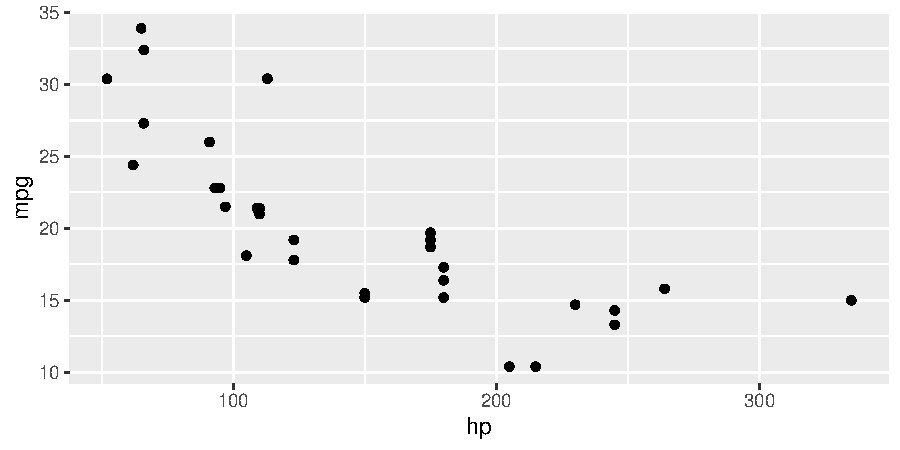
\includegraphics[width=0.95\linewidth]{figure/unnamed-chunk-2-1} 
\end{knitrout}
\end{frame}

\begin{frame}{ggplot2 structure from the "Cheat Sheet"}
\href{https://www.rstudio.com/resources/cheatsheets/}{Tidyverse Cheat Sheets including ggplot2}
\begin{figure}
  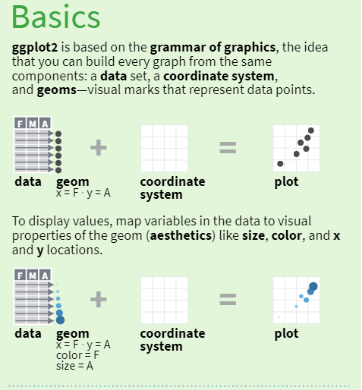
\includegraphics[height=0.75\textheight]{ggplot2cheatsheetbasic.png}
\end{figure}
\end{frame}

\begin{frame}{ggplot2 Options}

\href{https://ggplot2-book.org/}{ggplot2 book}
\begin{enumerate}
\item Plot types:  density, histogram, boxplot, bar chart, violin plot, error bars for bar plots, maps
\item custom color schemes, add fill/color or shapes matching categorical variables
\item custom scales or coordinate styems for continuous variables
\item faceting to make plots for each level of a categorical variable
\item custom labels and legends
\end{enumerate}

\end{frame}

\begin{frame}[fragile]{Example ggplot2 add facet and title}
\begin{knitrout}
\definecolor{shadecolor}{rgb}{0.969, 0.969, 0.969}\color{fgcolor}\begin{kframe}
\begin{alltt}
\hlstd{plotnew} \hlkwb{=} \hlstd{plot} \hlopt{+} \hlkwd{ggtitle}\hlstd{(}\hlstr{"MPG of Car given HP by
                         transmission"}\hlstd{)} \hlopt{+}
    \hlkwd{xlab}\hlstd{(}\hlstr{"Horse Power"}\hlstd{)} \hlopt{+} \hlkwd{ylab}\hlstd{(}\hlstr{"Miles Per Gallon"}\hlstd{)} \hlopt{+}
    \hlkwd{facet_grid}\hlstd{(}\hlopt{~}\hlstd{am)}
\end{alltt}
\end{kframe}
\end{knitrout}
\end{frame}


\begin{frame}[fragile]{Example ggplot2 add facet and title}
\begin{knitrout}
\definecolor{shadecolor}{rgb}{0.969, 0.969, 0.969}\color{fgcolor}\begin{kframe}
\begin{alltt}
\hlstd{plotnew}
\end{alltt}
\end{kframe}
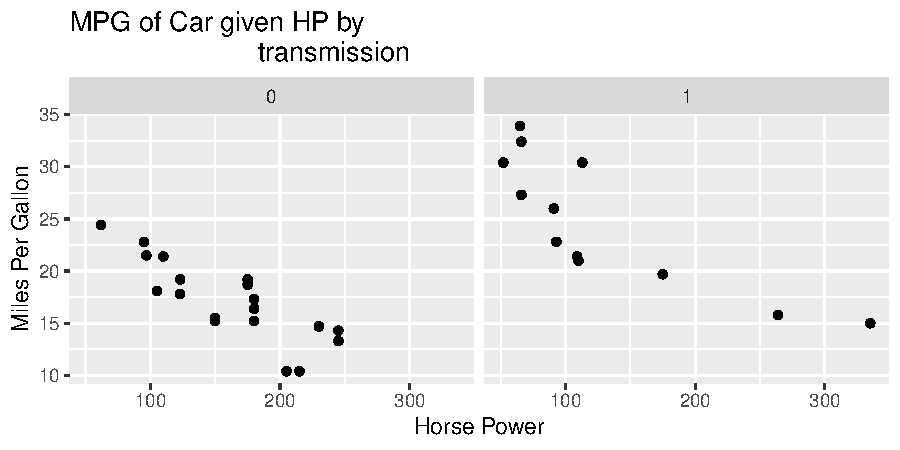
\includegraphics[width=0.95\linewidth]{figure/unnamed-chunk-4-1} 
\end{knitrout}
\end{frame}

\begin{frame}[fragile]{Why ggsurvey}
\begin{itemize}
\item ggplot2 has all the necessary components to make visualizations of survey data but the code can get messy especially when handling weights or making crosstabs.
\item ggplot2 defaults to showing categorical data via counts, but proportions are often of interest with survey data especially when making comparisons across groups of different size.
\item ggsurvey creates functions to make common visualizations of survey data in a single function call while preserving some of the customization features in ggplot.
\item ggsurvey retains the compatibility of ggplot2 with the rest of the tidyverse
\item ggsurvey has functions to handle data frames (with weight as a variable) and functions that handle svy.design objects from survey package.
\end{itemize}
\end{frame}

\begin{frame}{ggsurvey Features}
\begin{itemize}
\item ggsurvey plot types: bar chart, histogram, boxplot, hexplot
\item has faceting built in using 2d (one facets), 3d (two facets)
\item uses weight argument in ggplot to handle weights
\item ggsurvey is a series of "wrapper" functions that call ggplot or other tidyverse functions
\item ggsurvey works with unweighted data if you add a "weight" variable that is 1 for every row
\end{itemize}
\end{frame}

\begin{frame}[fragile]{Dataset 2: apistrat from the survey package}
The second dataset we will use is the apistrat data set from the survey package.  This a stratified sample from a data set of all California schools with various characteristics of the schools such as type of school (stype), the Academic Performance index in 1999 and 2000 (api99, api00), if a school is year round (yr.rnd), percent of parents that are high school graduates (hsg)
\begin{knitrout}
\definecolor{shadecolor}{rgb}{0.969, 0.969, 0.969}\color{fgcolor}\begin{kframe}
\begin{alltt}
\hlkwd{library}\hlstd{(survey)}
\hlkwd{data}\hlstd{(api)}
\hlkwd{library}\hlstd{(dplyr)}
\end{alltt}
\end{kframe}
\end{knitrout}
\end{frame}

\begin{frame}[fragile]{Example 2A Crosstabs with base ggplot}
By default, ggplot does not adjust for varying sample sizes across graphics which doesn't always lead to good comparisons.
\begin{knitrout}
\definecolor{shadecolor}{rgb}{0.969, 0.969, 0.969}\color{fgcolor}\begin{kframe}
\begin{alltt}
\hlkwd{ggplot}\hlstd{(apistrat,} \hlkwd{aes}\hlstd{(yr.rnd))} \hlopt{+}
    \hlkwd{geom_bar}\hlstd{(}\hlkwd{aes}\hlstd{(}\hlkwc{weight} \hlstd{= pw))} \hlopt{+}
    \hlkwd{facet_grid}\hlstd{(}\hlkwc{cols} \hlstd{=} \hlkwd{vars}\hlstd{(stype))}
\end{alltt}
\end{kframe}
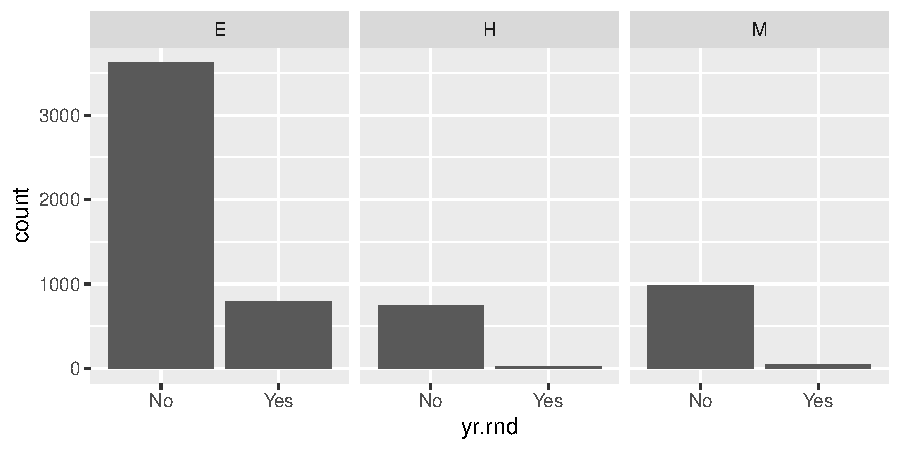
\includegraphics[width=0.95\linewidth]{figure/unnamed-chunk-6-1} 
\end{knitrout}
\end{frame}

\begin{frame}[fragile]{Example 2A Crosstabs with base ggplot}
First let's look at the base ggplot2 code needed to produce a crosstab.
\begin{knitrout}
\definecolor{shadecolor}{rgb}{0.969, 0.969, 0.969}\color{fgcolor}\begin{kframe}
\begin{alltt}
\hlstd{newdf} \hlkwb{=} \hlstd{apistrat} \hlopt
    \hlkwd{group_by}\hlstd{(stype, yr.rnd)} \hlopt
    \hlkwd{tally}\hlstd{(,} \hlkwc{wt} \hlstd{= pw)} \hlopt
    \hlkwd{mutate}\hlstd{(}\hlkwc{f} \hlstd{= n}\hlopt{/}\hlkwd{sum}\hlstd{(n))}
\hlstd{plotnew} \hlkwb{=} \hlkwd{ggplot}\hlstd{(newdf,} \hlkwd{aes}\hlstd{(yr.rnd))} \hlopt{+}
    \hlkwd{geom_bar}\hlstd{(}\hlkwd{aes}\hlstd{(}\hlkwc{weight} \hlstd{= f))} \hlopt{+}
    \hlkwd{facet_grid}\hlstd{(}\hlkwc{cols} \hlstd{=} \hlkwd{vars}\hlstd{(stype))}
\end{alltt}
\end{kframe}
\end{knitrout}
\end{frame}

\begin{frame}[fragile]{Example 2A Crosstabs with base ggplot}
First let's look at the base ggplot2 code needed to produce a crosstab.
\begin{knitrout}
\definecolor{shadecolor}{rgb}{0.969, 0.969, 0.969}\color{fgcolor}\begin{kframe}
\begin{alltt}
\hlstd{plotnew}
\end{alltt}
\end{kframe}
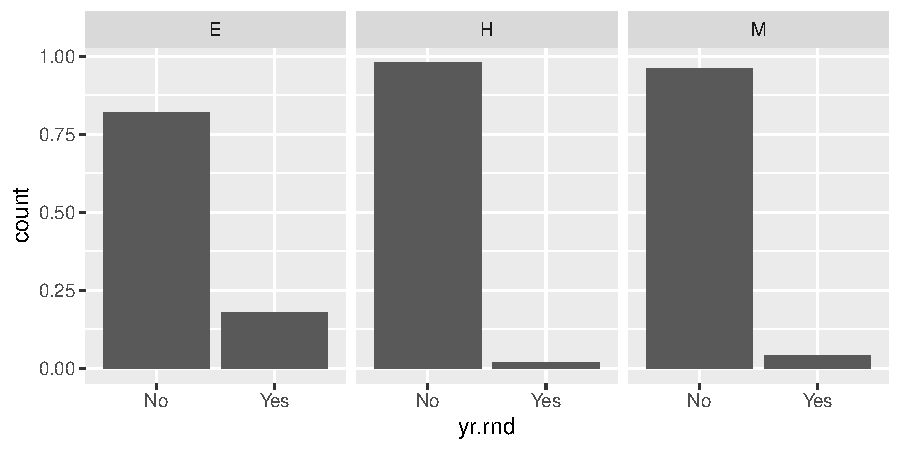
\includegraphics[width=0.95\linewidth]{figure/unnamed-chunk-8-1} 
\end{knitrout}
\end{frame}

\begin{frame}[fragile]{Example 2B Crosstabs with ggsurvey}
\begin{knitrout}
\definecolor{shadecolor}{rgb}{0.969, 0.969, 0.969}\color{fgcolor}\begin{kframe}
\begin{alltt}
\hlkwd{library}\hlstd{(ggsurvey)}
\hlkwd{ggbarcrosstabs}\hlstd{(apistrat, yr.rnd,}
    \hlstd{stype, pw)}
\end{alltt}
\end{kframe}
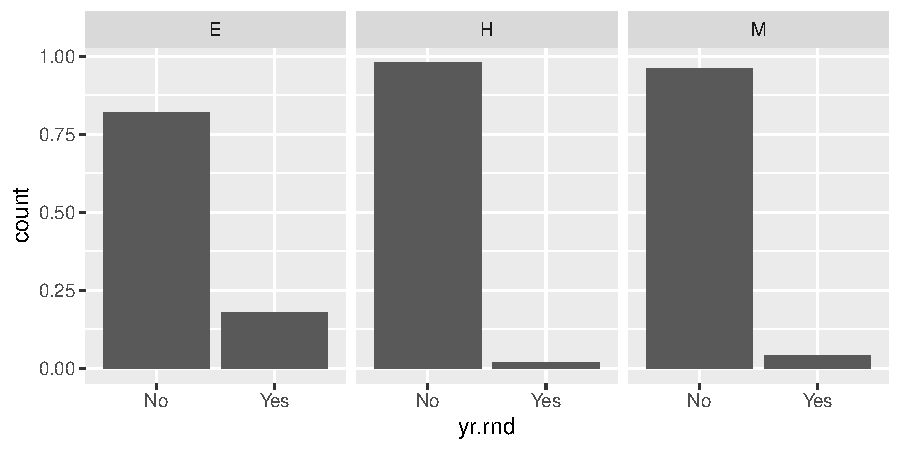
\includegraphics[width=0.95\linewidth]{figure/unnamed-chunk-9-1} 
\end{knitrout}
\end{frame}


\section{Using ggplot2}
\begin{frame}
To understand the what can be done with ggsurvey, we will first look at how base ggplot2 works for non-survey data.\\
In base ggplot2 a plot is made with at least two functions: ggplot and an appriorate geom function.  There are some geoms that are commonly used in addition to other geoms such as adding text or error bars.
\end{frame}

\begin{frame}[fragile]{Main Plot Geoms}

\begin{table}[]
\begin{tabular}{|l|l|}
\hline
            & Geom function                                                                                        \\ \hline
Bar chart   & \begin{tabular}[c]{@{}l@{}}geom\_bar (for raw data), \\ geom\_col (for frequency tables)\end{tabular} \\ \hline
Boxplot     & geom\_boxplot                                                                                         \\ \hline
Histogram   & geom\_histogram                                                                                       \\ \hline
Line Plot   & geom\_line                                                                                            \\ \hline
Scatterplot & geom\_point                                                                                          \\ \hline
Hex plot    & geom\_hexbin (in hexbin package)                                                                      \\ \hline
Violin plot & geom\_violin                                                                                          \\ \hline
\end{tabular}
\end{table}
\end{frame}

\begin{frame}[fragile]{Supplemental Plot Geoms}
\begin{table}[]
\begin{tabular}{|l|l|}
\hline
                & Geom            \\ \hline
Error bars      & geom\_errorbars \\ \hline
Text            & geom\_text      \\ \hline
Smoothing lines & geom\_smooth    \\ \hline
Line            & geom\_abline    \\ \hline
horizontal line & geom\_hline     \\ \hline
vertical line   & geom\_vline     \\ \hline
\end{tabular}
\end{table}
\end{frame}


\begin{frame}[fragile]{Dataset 3:  Palmer Penguins}
The Palmer penguins data set details information taken from penguins on the palmer archipelago.  The variables are
species, island, bill\_length\_mm, bill\_depth\_mm, flipper\_depth\_mm, flipper\_length\_mm, body\_mass\_g, sex, year.
\begin{knitrout}
\definecolor{shadecolor}{rgb}{0.969, 0.969, 0.969}\color{fgcolor}\begin{kframe}
\begin{alltt}
\hlkwd{library}\hlstd{(palmerpenguins)}
\hlkwd{data}\hlstd{(penguins)}
\end{alltt}
\end{kframe}
\end{knitrout}
\end{frame}

\begin{frame}[fragile]{Example 3: A Bar Chart}
First let's use the ggplot and geom\_bar functions to make a bar chart of the species of penguins in the data set.
\begin{knitrout}
\definecolor{shadecolor}{rgb}{0.969, 0.969, 0.969}\color{fgcolor}\begin{kframe}
\begin{alltt}
\hlstd{plot3} \hlkwb{=} \hlkwd{ggplot}\hlstd{(penguins,} \hlkwd{aes}\hlstd{(species))} \hlopt{+}
    \hlkwd{geom_bar}\hlstd{()}
\hlstd{plot3}
\end{alltt}
\end{kframe}
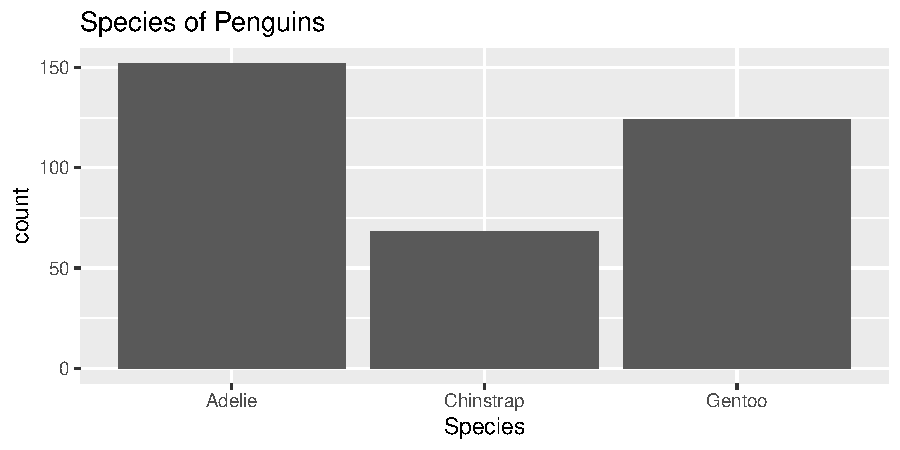
\includegraphics[width=0.95\linewidth]{figure/unnamed-chunk-11-1} 
\end{knitrout}

\end{frame}



\begin{frame}[fragile]{Title customization for Example 3}
Next let's add a title to the previous plot with ggtitle.
\begin{knitrout}
\definecolor{shadecolor}{rgb}{0.969, 0.969, 0.969}\color{fgcolor}\begin{kframe}
\begin{alltt}
\hlstd{plot3} \hlopt{+} \hlkwd{ggtitle}\hlstd{(}\hlstr{"Species of Penguins"}\hlstd{)}
\end{alltt}
\end{kframe}
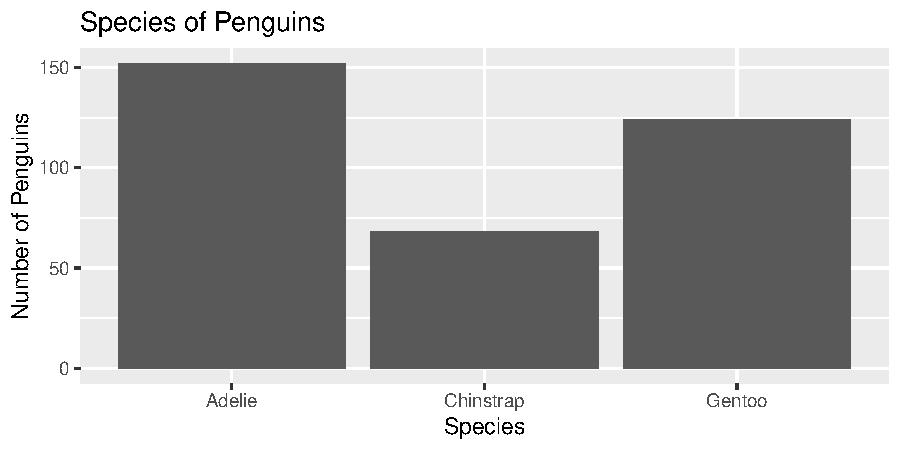
\includegraphics[width=0.95\linewidth]{figure/unnamed-chunk-12-1} 
\end{knitrout}
\end{frame}


\begin{frame}[fragile]{Label customization Part 1 for Example 3}
Next let's add a x axis label  with  xlab adds a label to the x axis.
\begin{knitrout}
\definecolor{shadecolor}{rgb}{0.969, 0.969, 0.969}\color{fgcolor}\begin{kframe}
\begin{alltt}
\hlstd{plot3} \hlopt{+} \hlkwd{ggtitle}\hlstd{(}\hlstr{"Species of Penguins"}\hlstd{)} \hlopt{+}
    \hlkwd{xlab}\hlstd{(}\hlstr{"Species"}\hlstd{)}
\end{alltt}
\end{kframe}
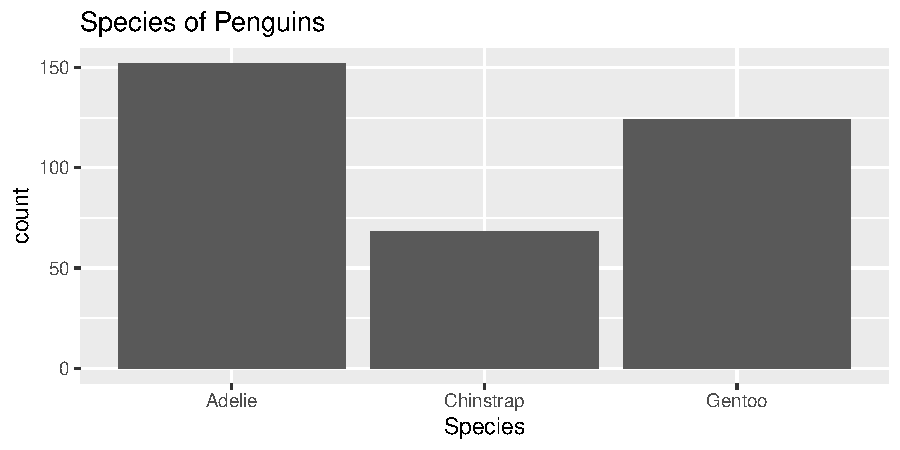
\includegraphics[width=0.95\linewidth]{figure/unnamed-chunk-13-1} 
\end{knitrout}
\end{frame}
\begin{frame}[fragile]{Label customization Part 2 for Example 3}
Next let's add a y axis label to the previous plot with ylab.
\begin{knitrout}
\definecolor{shadecolor}{rgb}{0.969, 0.969, 0.969}\color{fgcolor}\begin{kframe}
\begin{alltt}
\hlstd{plot3title} \hlkwb{=} \hlstd{plot3} \hlopt{+} \hlkwd{ggtitle}\hlstd{(}\hlstr{"Species of Penguins"}\hlstd{)} \hlopt{+}
    \hlkwd{xlab}\hlstd{(}\hlstr{"Species"}\hlstd{)} \hlopt{+} \hlkwd{ylab}\hlstd{(}\hlstr{"Number of Penguins"}\hlstd{)}
\hlstd{plot3title}
\end{alltt}
\end{kframe}
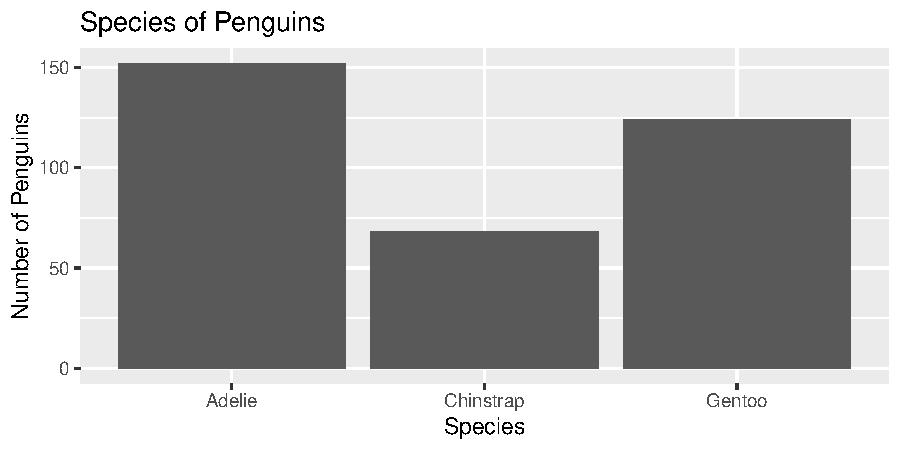
\includegraphics[width=0.95\linewidth]{figure/unnamed-chunk-14-1} 
\end{knitrout}
\end{frame}

\begin{frame}[fragile]{Label customization Part 2 for Example 3}
Next let's add a y axis label to the previous plot with ylab.
\begin{knitrout}
\definecolor{shadecolor}{rgb}{0.969, 0.969, 0.969}\color{fgcolor}\begin{kframe}
\begin{alltt}
\hlstd{plot3title}
\end{alltt}
\end{kframe}
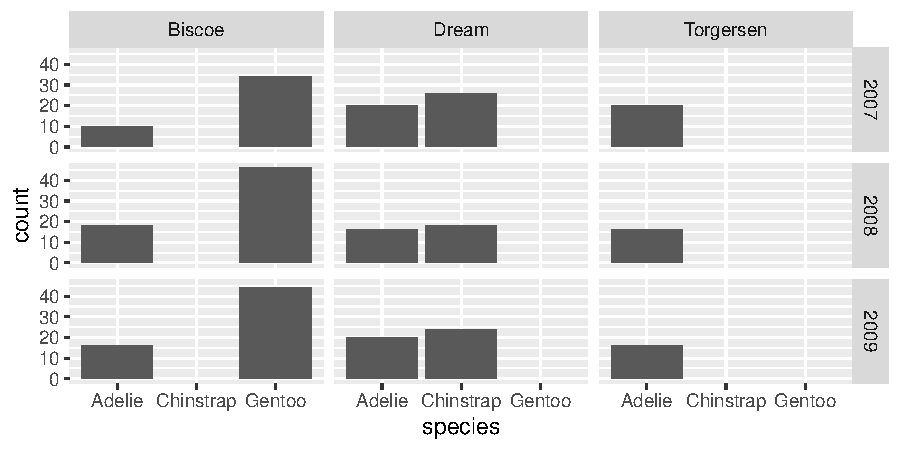
\includegraphics[width=0.95\linewidth]{figure/unnamed-chunk-15-1} 
\end{knitrout}
\end{frame}
\begin{frame}[fragile]{Color customization}
We can make the bars each a different color by passing aes(fill = Species) inside geom\_bar
\begin{knitrout}
\definecolor{shadecolor}{rgb}{0.969, 0.969, 0.969}\color{fgcolor}\begin{kframe}
\begin{alltt}
\hlstd{plot3color} \hlkwb{=} \hlkwd{ggplot}\hlstd{(penguins,} \hlkwd{aes}\hlstd{(species))} \hlopt{+}
    \hlkwd{geom_bar}\hlstd{(}\hlkwd{aes}\hlstd{(}\hlkwc{fill} \hlstd{= species))} \hlopt{+}
    \hlkwd{ggtitle}\hlstd{(}\hlstr{"Species of Penguins"}\hlstd{)} \hlopt{+}
    \hlkwd{xlab}\hlstd{(}\hlstr{"Species"}\hlstd{)} \hlopt{+} \hlkwd{ylab}\hlstd{(}\hlstr{"Number of Penguins"}\hlstd{)}
\end{alltt}
\end{kframe}
\end{knitrout}
\end{frame}

\begin{frame}[fragile]{Color customization}
We can make the bars each a different color by passing aes(fill = Species) inside geom\_bar
\begin{knitrout}
\definecolor{shadecolor}{rgb}{0.969, 0.969, 0.969}\color{fgcolor}\begin{kframe}
\begin{alltt}
\hlstd{plot3color}
\end{alltt}
\end{kframe}
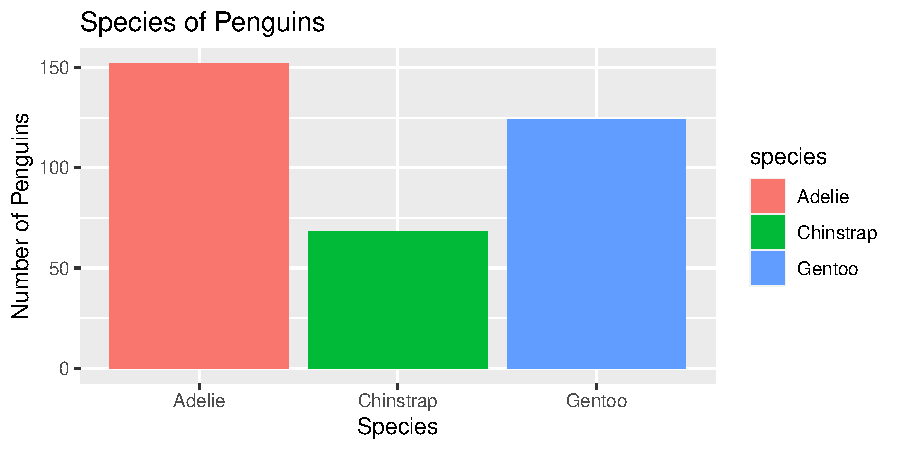
\includegraphics[width=0.95\linewidth]{figure/unnamed-chunk-17-1} 
\end{knitrout}
\end{frame}

\begin{frame}[fragile]{Faceting}
Faceting is a common tool to compare the the distribution of one set of variables by considering another variable. Going back to Example 1, we compared the relationship between horsepower and mpg depending on the transmission of the car using facet\_grid. Faceting helps to show the affect of a variable on multiple variables.  Crosstabs are faceted graphs comparing the distribution of a survey question given an categorical variable.
\end{frame}

\begin{frame}[fragile]{Faceting}

\begin{knitrout}
\definecolor{shadecolor}{rgb}{0.969, 0.969, 0.969}\color{fgcolor}\begin{kframe}
\begin{alltt}
\hlstd{plotnew} \hlkwb{=} \hlstd{plot} \hlopt{+} \hlkwd{ggtitle}\hlstd{(}\hlstr{"MPG of Car given HP by
                         transmission"}\hlstd{)} \hlopt{+}
    \hlkwd{xlab}\hlstd{(}\hlstr{"Horse Power"}\hlstd{)} \hlopt{+} \hlkwd{ylab}\hlstd{(}\hlstr{"Miles Per Gallon"}\hlstd{)} \hlopt{+}
    \hlkwd{facet_grid}\hlstd{(}\hlopt{~}\hlstd{am)}
\end{alltt}
\end{kframe}
\end{knitrout}
\end{frame}


\begin{frame}[fragile]{Example 4 Bar chart of Species with Facet Grid}
$y~x$ means x is on the horizontal axis
\begin{knitrout}
\definecolor{shadecolor}{rgb}{0.969, 0.969, 0.969}\color{fgcolor}\begin{kframe}
\begin{alltt}
\hlstd{plot4} \hlkwb{=} \hlkwd{ggplot}\hlstd{(penguins,} \hlkwd{aes}\hlstd{(species))} \hlopt{+}
    \hlkwd{geom_bar}\hlstd{()} \hlopt{+} \hlkwd{facet_grid}\hlstd{(year} \hlopt{~}
    \hlstd{island)}
\hlstd{plot4}
\end{alltt}
\end{kframe}
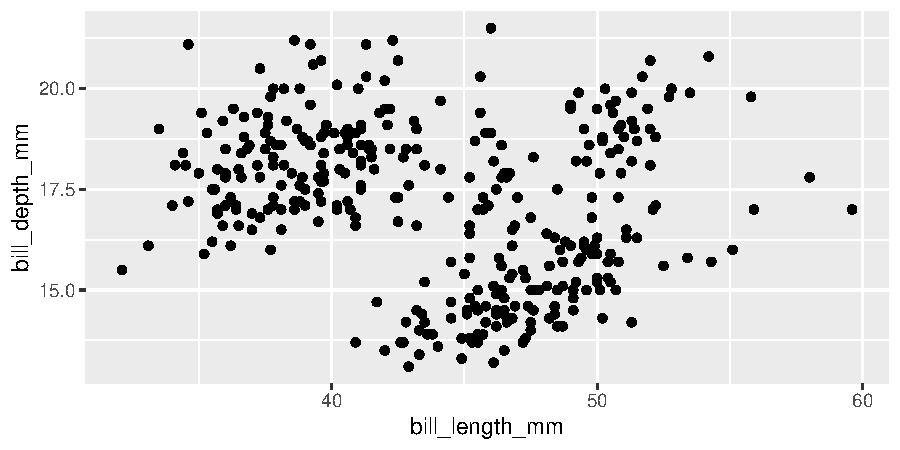
\includegraphics[width=0.95\linewidth]{figure/unnamed-chunk-19-1} 
\end{knitrout}
\end{frame}

\begin{frame}[fragile]{Example 4 Bar chart of Species with Facet Grid}
\begin{knitrout}
\definecolor{shadecolor}{rgb}{0.969, 0.969, 0.969}\color{fgcolor}\begin{kframe}
\begin{alltt}
\hlstd{plot4}
\end{alltt}
\end{kframe}
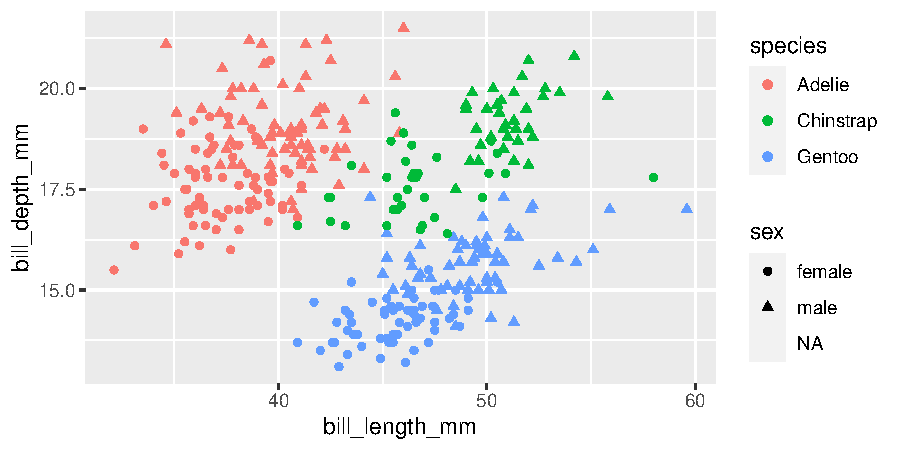
\includegraphics[width=0.95\linewidth]{figure/unnamed-chunk-20-1} 
\end{knitrout}
\end{frame}

\begin{frame}[fragile]{Example 4 Bar chart of Species with Facet Grid}
\begin{knitrout}
\definecolor{shadecolor}{rgb}{0.969, 0.969, 0.969}\color{fgcolor}\begin{kframe}
\begin{alltt}
\hlstd{plot4a} \hlkwb{=} \hlkwd{ggplot}\hlstd{(penguins,} \hlkwd{aes}\hlstd{(species))} \hlopt{+}
    \hlkwd{geom_bar}\hlstd{()} \hlopt{+} \hlkwd{facet_grid}\hlstd{(}\hlkwc{rows} \hlstd{=} \hlkwd{vars}\hlstd{(year),}
    \hlkwc{cols} \hlstd{=} \hlkwd{vars}\hlstd{(island))}
\end{alltt}
\end{kframe}
\end{knitrout}
\end{frame}

\begin{frame}[fragile]{Example 4 Bar chart of Species with Facet Grid }
\begin{knitrout}
\definecolor{shadecolor}{rgb}{0.969, 0.969, 0.969}\color{fgcolor}\begin{kframe}
\begin{alltt}
\hlstd{plot4a}
\end{alltt}
\end{kframe}
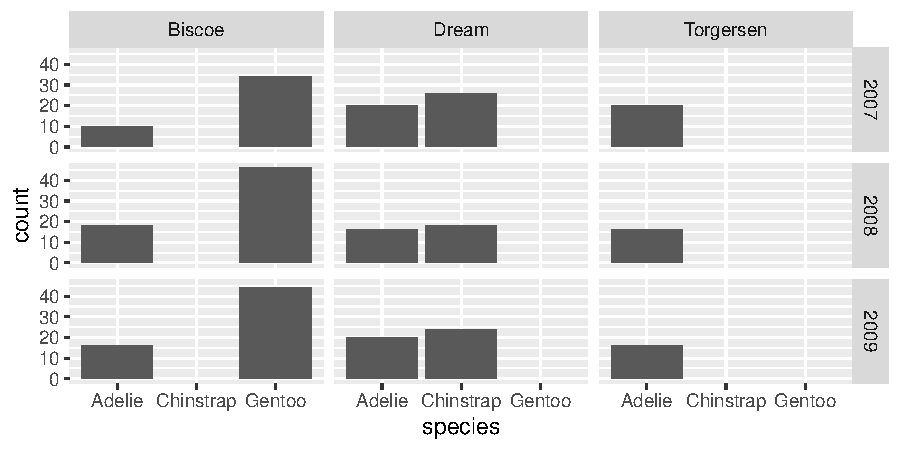
\includegraphics[width=0.95\linewidth]{figure/unnamed-chunk-22-1} 
\end{knitrout}
\end{frame}
\begin{frame}[fragile]{Example 4 Bar chart text wrapping }
\begin{knitrout}
\definecolor{shadecolor}{rgb}{0.969, 0.969, 0.969}\color{fgcolor}\begin{kframe}
\begin{alltt}
\hlkwd{library}\hlstd{(ggrepel)}
\hlstd{plot4} \hlopt{+} \hlkwd{theme}\hlstd{(}\hlkwc{axis.text.x} \hlstd{=} \hlkwd{element_text}\hlstd{(}\hlkwc{angle} \hlstd{=} \hlnum{45}\hlstd{,}
    \hlkwc{hjust} \hlstd{=} \hlnum{1}\hlstd{))}
\end{alltt}
\end{kframe}
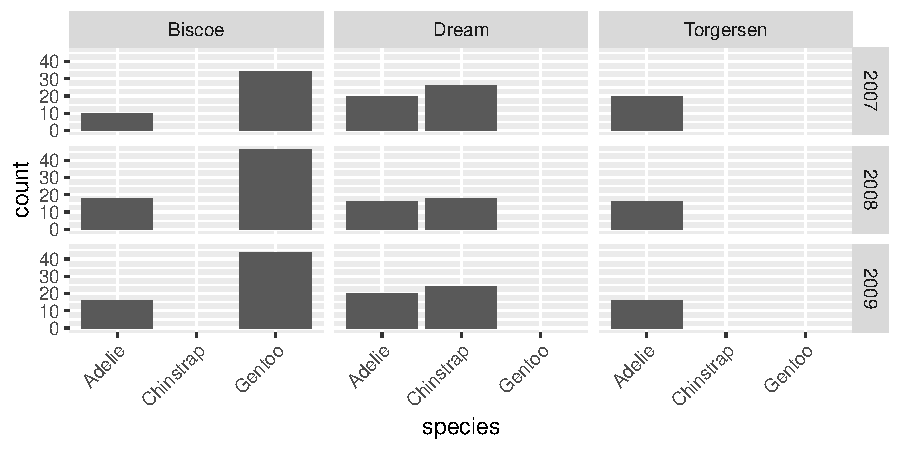
\includegraphics[width=0.95\linewidth]{figure/unnamed-chunk-23-1} 
\end{knitrout}
\end{frame}

\begin{frame}[fragile]{Facet Wrap}
Facet Wrap wraps the facet for when there are too many columns/rows
\begin{knitrout}
\definecolor{shadecolor}{rgb}{0.969, 0.969, 0.969}\color{fgcolor}\begin{kframe}
\begin{alltt}
\hlstd{plot4} \hlkwb{=} \hlkwd{ggplot}\hlstd{(penguins,} \hlkwd{aes}\hlstd{(species))} \hlopt{+}
    \hlkwd{geom_bar}\hlstd{()} \hlopt{+} \hlkwd{facet_wrap}\hlstd{(}\hlkwd{vars}\hlstd{(year,}
    \hlstd{island))}
\end{alltt}
\end{kframe}
\end{knitrout}

\end{frame}

\begin{frame}[fragile]{Facet Wrap}
\begin{knitrout}
\definecolor{shadecolor}{rgb}{0.969, 0.969, 0.969}\color{fgcolor}\begin{kframe}
\begin{alltt}
\hlstd{plot4}
\end{alltt}
\end{kframe}
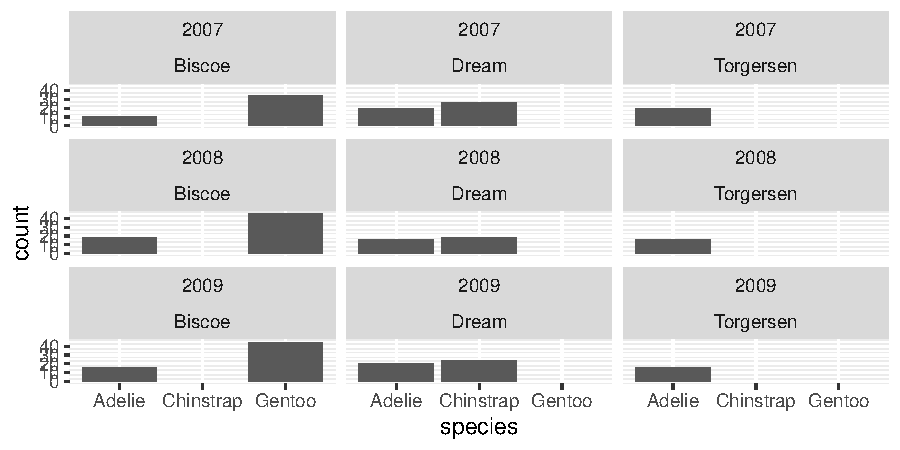
\includegraphics[width=0.95\linewidth]{figure/unnamed-chunk-25-1} 
\end{knitrout}

\end{frame}

\begin{frame}[fragile]{Example 5 Scatterplots}
\begin{knitrout}
\definecolor{shadecolor}{rgb}{0.969, 0.969, 0.969}\color{fgcolor}\begin{kframe}
\begin{alltt}
\hlstd{plot5} \hlkwb{=} \hlkwd{ggplot}\hlstd{(penguins,} \hlkwd{aes}\hlstd{(}\hlkwc{x} \hlstd{= bill_length_mm,}
    \hlkwc{y} \hlstd{= bill_depth_mm))} \hlopt{+} \hlkwd{geom_point}\hlstd{()}
\end{alltt}
\end{kframe}
\end{knitrout}

\end{frame}

\begin{frame}[fragile]{Example 5 Scatterplots}
\begin{knitrout}
\definecolor{shadecolor}{rgb}{0.969, 0.969, 0.969}\color{fgcolor}\begin{kframe}
\begin{alltt}
\hlstd{plot5}
\end{alltt}
\end{kframe}
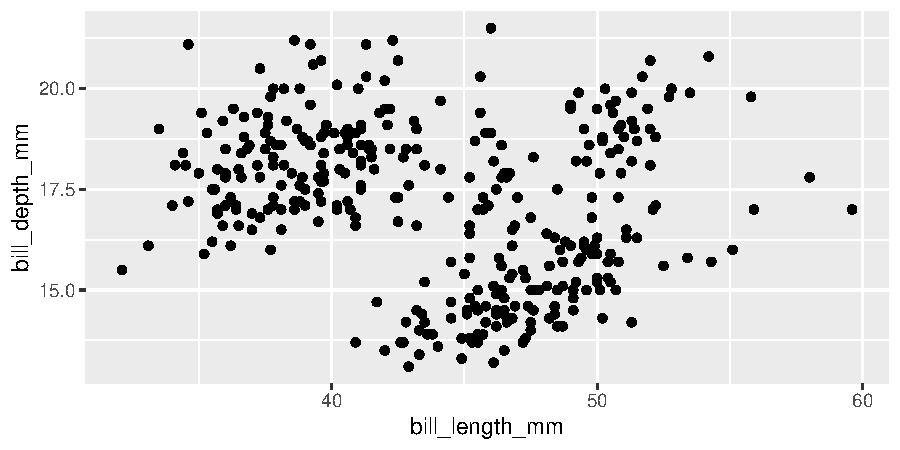
\includegraphics[width=0.95\linewidth]{figure/unnamed-chunk-27-1} 
\end{knitrout}

\end{frame}
\begin{frame}[fragile]{Example 5 with Species and Sex}
\begin{knitrout}
\definecolor{shadecolor}{rgb}{0.969, 0.969, 0.969}\color{fgcolor}\begin{kframe}
\begin{alltt}
\hlstd{plot5a} \hlkwb{=} \hlkwd{ggplot}\hlstd{(penguins,} \hlkwd{aes}\hlstd{(}\hlkwc{x} \hlstd{= bill_length_mm,}
    \hlkwc{y} \hlstd{= bill_depth_mm))} \hlopt{+} \hlkwd{geom_point}\hlstd{(}\hlkwd{aes}\hlstd{(}\hlkwc{color} \hlstd{= species,}
    \hlkwc{shape} \hlstd{= sex))}
\end{alltt}
\end{kframe}
\end{knitrout}

\end{frame}

\begin{frame}[fragile]{Example 5 with Species and Sex}
\begin{knitrout}
\definecolor{shadecolor}{rgb}{0.969, 0.969, 0.969}\color{fgcolor}\begin{kframe}
\begin{alltt}
\hlstd{plot5a}
\end{alltt}
\end{kframe}
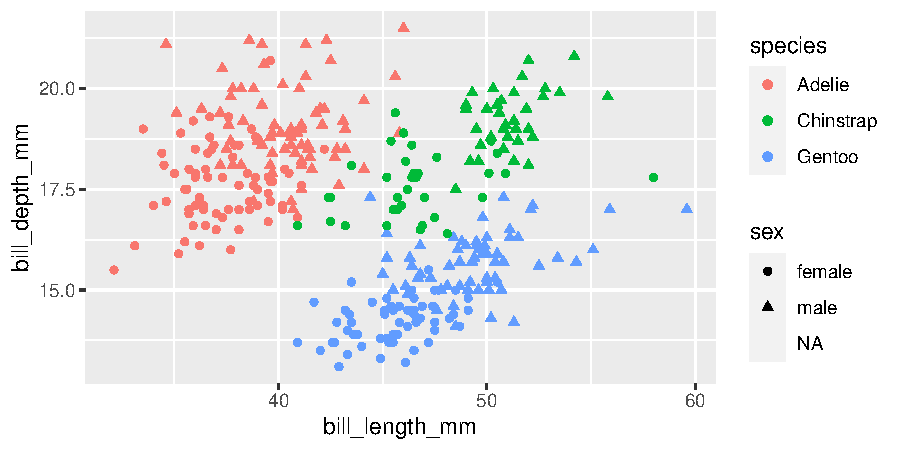
\includegraphics[width=0.95\linewidth]{figure/unnamed-chunk-29-1} 
\end{knitrout}

\end{frame}

\begin{frame}[fragile]{Example 6A Histograms}
A histogram takes a continuous variable and puts it into bins and then counts the number of data points in each bin.By default geom\_histogram makes 30 evenly sized bins.
\begin{knitrout}
\definecolor{shadecolor}{rgb}{0.969, 0.969, 0.969}\color{fgcolor}\begin{kframe}
\begin{alltt}
\hlkwd{ggplot}\hlstd{(penguins,} \hlkwd{aes}\hlstd{(}\hlkwc{x} \hlstd{= body_mass_g))} \hlopt{+}
    \hlkwd{geom_histogram}\hlstd{()}
\end{alltt}
\end{kframe}
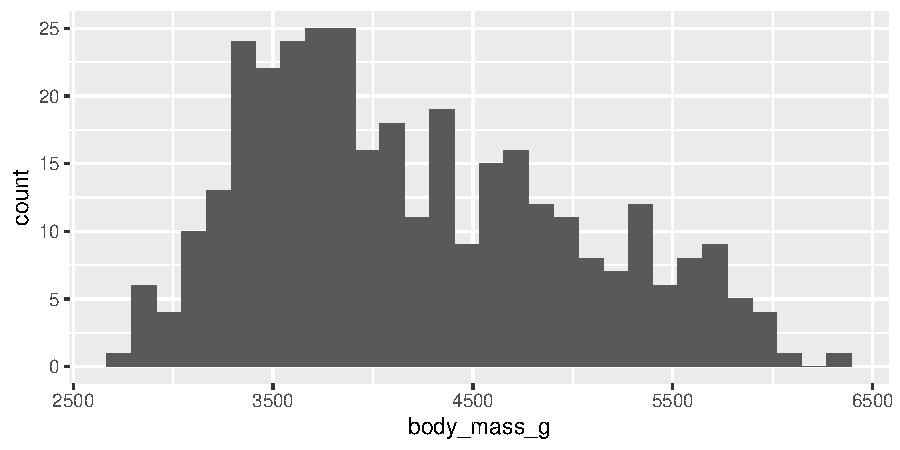
\includegraphics[width=0.95\linewidth]{figure/unnamed-chunk-30-1} 
\end{knitrout}


\end{frame}

\begin{frame}[fragile]{Example 6B Histograms}
We can specify the size of the bins with binwidth. I prefer to try the default bins to get a sense of the range of the data.
\begin{knitrout}
\definecolor{shadecolor}{rgb}{0.969, 0.969, 0.969}\color{fgcolor}\begin{kframe}
\begin{alltt}
\hlstd{plot6b} \hlkwb{=} \hlkwd{ggplot}\hlstd{(penguins,} \hlkwd{aes}\hlstd{(}\hlkwc{x} \hlstd{= body_mass_g))} \hlopt{+}
    \hlkwd{geom_histogram}\hlstd{(}\hlkwc{binwidth} \hlstd{=} \hlnum{200}\hlstd{)}
\end{alltt}
\end{kframe}
\end{knitrout}


\end{frame}


\begin{frame}[fragile]{Example 6B Histograms}
We can specify the size of the bins with binwidth. I prefer to try the default bins to get a sense of the range of the data.
\begin{knitrout}
\definecolor{shadecolor}{rgb}{0.969, 0.969, 0.969}\color{fgcolor}\begin{kframe}
\begin{alltt}
\hlstd{plot6b}
\end{alltt}
\end{kframe}
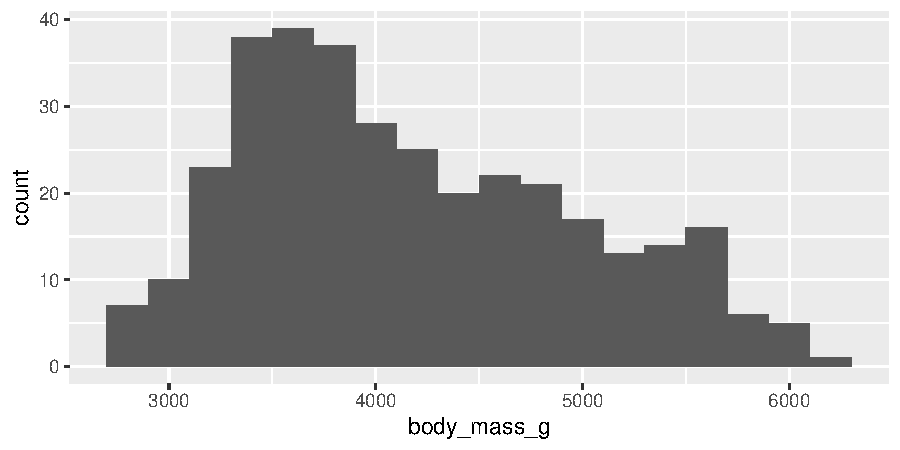
\includegraphics[width=0.95\linewidth]{figure/unnamed-chunk-32-1} 
\end{knitrout}


\end{frame}
\begin{frame}[fragile]{Example 7 Boxplot}
A boxplot shows the minimum, 25th percentile, median, 75th percentile, and maximum.
\begin{knitrout}
\definecolor{shadecolor}{rgb}{0.969, 0.969, 0.969}\color{fgcolor}\begin{kframe}
\begin{alltt}
\hlkwd{ggplot}\hlstd{(penguins,} \hlkwd{aes}\hlstd{(}\hlkwc{x} \hlstd{= flipper_length_mm))} \hlopt{+}
    \hlkwd{geom_boxplot}\hlstd{()}
\end{alltt}
\end{kframe}
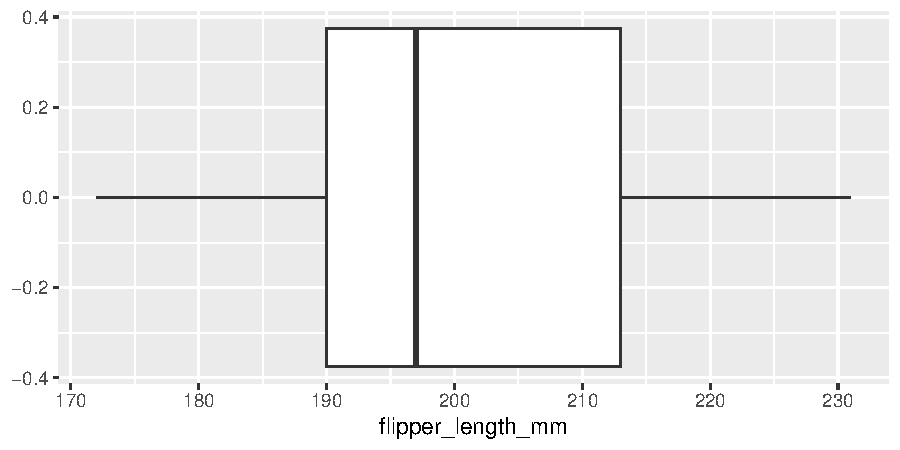
\includegraphics[width=0.95\linewidth]{figure/unnamed-chunk-33-1} 
\end{knitrout}

\end{frame}

\begin{frame}[fragile]{Example 7 Boxplot by Species}
\begin{knitrout}
\definecolor{shadecolor}{rgb}{0.969, 0.969, 0.969}\color{fgcolor}\begin{kframe}
\begin{alltt}
\hlstd{plot7} \hlkwb{=} \hlkwd{ggplot}\hlstd{(penguins,} \hlkwd{aes}\hlstd{(}\hlkwc{x} \hlstd{= flipper_length_mm,}
    \hlkwc{y} \hlstd{= species))} \hlopt{+} \hlkwd{geom_boxplot}\hlstd{()}
\end{alltt}
\end{kframe}
\end{knitrout}

\end{frame}

\begin{frame}[fragile]{Example 7 Boxplot by Species}
\begin{knitrout}
\definecolor{shadecolor}{rgb}{0.969, 0.969, 0.969}\color{fgcolor}\begin{kframe}
\begin{alltt}
\hlstd{plot7}
\end{alltt}
\end{kframe}
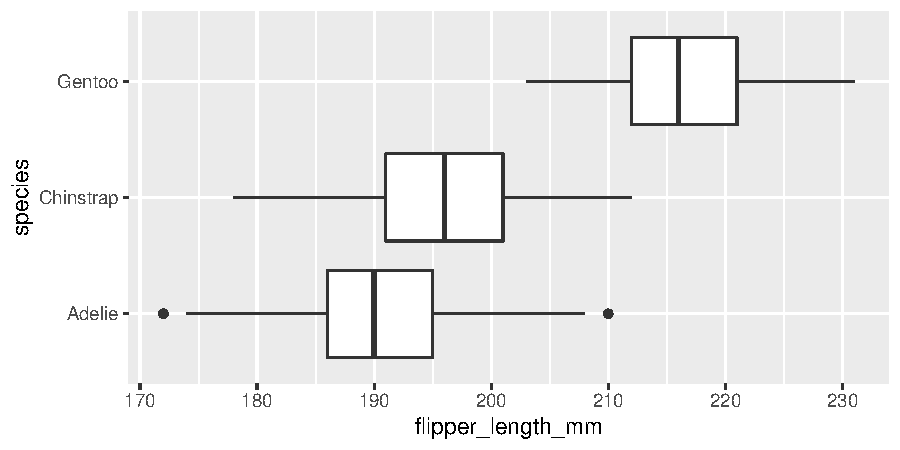
\includegraphics[width=0.95\linewidth]{figure/unnamed-chunk-35-1} 
\end{knitrout}

\end{frame}
\begin{frame}[fragile]{Example 7 with Title}
\begin{knitrout}
\definecolor{shadecolor}{rgb}{0.969, 0.969, 0.969}\color{fgcolor}\begin{kframe}
\begin{alltt}
\hlstd{plot7new} \hlkwb{=} \hlstd{plot7} \hlopt{+} \hlkwd{ggtitle}\hlstd{(}\hlstr{"Boxplot of Flipper Length"}\hlstd{)} \hlopt{+}
    \hlkwd{xlab}\hlstd{(}\hlstr{"Flipper Length"}\hlstd{)} \hlopt{+} \hlkwd{ylab}\hlstd{(}\hlstr{"Species"}\hlstd{)}
\hlstd{plot7new}
\end{alltt}
\end{kframe}
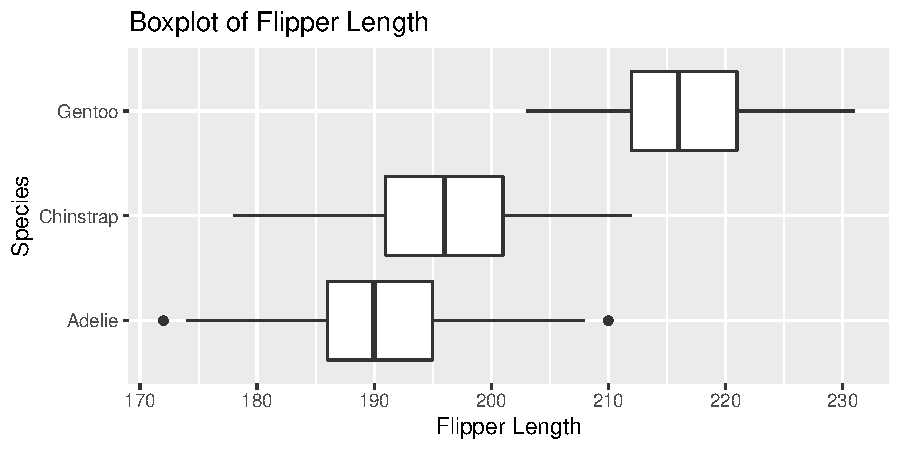
\includegraphics[width=0.95\linewidth]{figure/unnamed-chunk-36-1} 
\end{knitrout}

\end{frame}

\begin{frame}[fragile]{Example 7 with Title}
\begin{knitrout}
\definecolor{shadecolor}{rgb}{0.969, 0.969, 0.969}\color{fgcolor}\begin{kframe}
\begin{alltt}
\hlstd{plot7new}
\end{alltt}
\end{kframe}
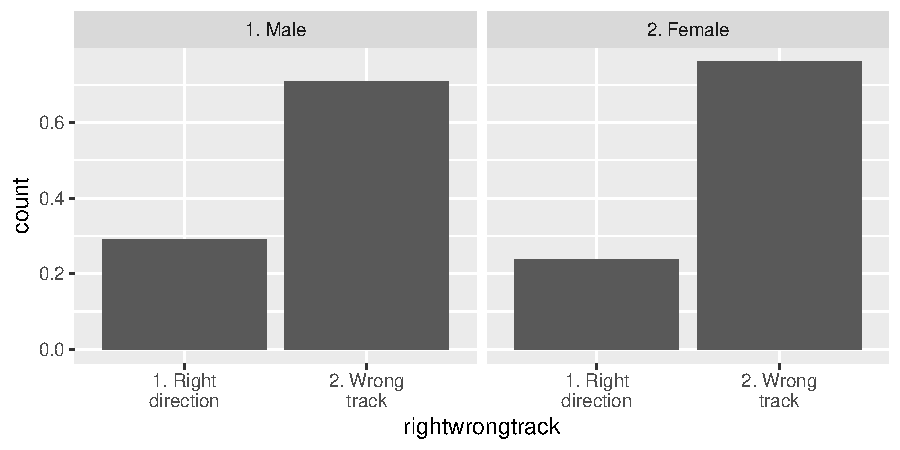
\includegraphics[width=0.95\linewidth]{figure/unnamed-chunk-37-1} 
\end{knitrout}

\end{frame}

\begin{frame}[fragile]{Example 7 with Facet for Year}
\begin{knitrout}
\definecolor{shadecolor}{rgb}{0.969, 0.969, 0.969}\color{fgcolor}\begin{kframe}
\begin{alltt}
\hlstd{plot7new} \hlopt{+} \hlkwd{facet_grid}\hlstd{(}\hlopt{~}\hlstd{year)}
\end{alltt}
\end{kframe}
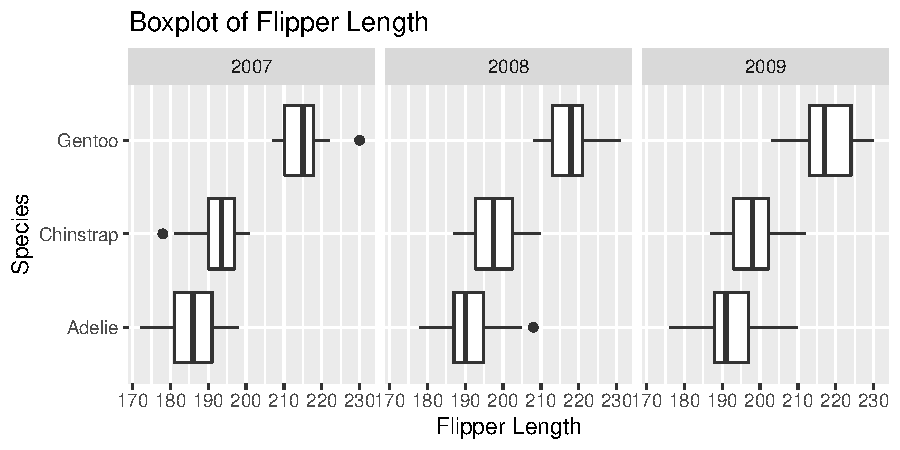
\includegraphics[width=0.95\linewidth]{figure/unnamed-chunk-38-1} 
\end{knitrout}
\end{frame}

\begin{frame}{Any Questions?}
\end{frame}
\section{Using ggsurvey for bar charts}
\begin{frame}{Introduction to ggsurvey vs ggplot}
\begin{itemize}
\item ggsurvey combines the ggplot+geom+facet\_grid into one function to save time
\item For each plot type ggsurvey specifies how to do it without a facet, with one facet, and with two facets
\item You can add ggtitle, xlab, ylab just like regular ggplot2
\item ggsurvey is compatible with dataframe and survey design objects (including srvyr objects for select functions)
\item like in ggplot we don't put column names in quotes
\item For data frames the survey weight should a column in the data frame
\end{itemize}
\end{frame}

\begin{frame}{Bar Chart Functions}
\begin{table}[]
\begin{tabular}{|l|l|l|}
\hline
Plot type                                                             & Data type  & ggsurvey function                                   \\ \hline
Bar Chart                                                             & data frame & ggbarweight(df, x, weights, fill)                   \\ \hline
Bar Chart                                                             & svydesign  & ggbarweight\_svy(surveyobj, x, fill)      \\ \hline
Crosstab                                                              & data frame & ggcrosstab(df, x, y,weights, fill, labeller)                  \\ \hline
Crosstab                                                              & svydesign  & ggcrosstab\_svy(surveyobj, x, y, fill, labeller)    \\ \hline
\begin{tabular}[c]{@{}l@{}}Crosstab\\ with 2\\ variables\end{tabular} & data frame & ggcrosstab3d(df, x, y,z weights, fill, labeller)    \\ \hline
\begin{tabular}[c]{@{}l@{}}Crosstab\\ with 2\\ variables\end{tabular} & svydesign  & ggcrosstab3d\_svy(surveyobj, x,y,z, fill. labeller) \\ \hline
\end{tabular}
\end{table}
\end{frame}

\begin{frame}{Dataset 4: ANES}
The American National Election Study is a large multi-mode multi-wave national survey conducted every two years with a broad range of questions related both to elections and broader policy issues. It is a collaboration between Stanford University and the University of Michigan and is funded by the National Science Foundation. It has been conducted since 1948. The population for the survey is US citizens.  \\
\href{https://electionstudies.org/}{ANES information}
The anesr package accesses ANES data, and we will use the 2020 time series data which has 8280 respondents.
\end{frame}

\begin{frame}[fragile]{Install and Load ANES}
\begin{knitrout}
\definecolor{shadecolor}{rgb}{0.969, 0.969, 0.969}\color{fgcolor}\begin{kframe}
\begin{alltt}
\hlcom{# install.packages('devtools')}
\hlcom{# library(devtools)}
\hlcom{# install_github('jamesmartherus/anesr')}
\hlkwd{library}\hlstd{(anesr)}
\hlkwd{data}\hlstd{(}\hlstr{"timeseries_2020"}\hlstd{)}
\hlstd{timeseries_2020} \hlkwb{=} \hlstd{haven}\hlopt{::}\hlkwd{as_factor}\hlstd{(timeseries_2020)}
\end{alltt}
\end{kframe}
\end{knitrout}
\end{frame}


\begin{frame}{Variables in ANES}
We will look at the following questions in the pre-election phase:  V201114 (Right Track / Wrong Track), V201390  (Speed of Response of Federal Government to COVID-19), V201324 (State of Economy), V201151 feeling thermometer for Joe Biden, V201152 feeling thermometer for Trump. \\
We will also consider crosstabs on the following variables  V201549x (race), V201511x (education), V201600 (gender). \\
The relevant weight is V200010a,strata V200010d, cluster is V200010c.
\end{frame}

\begin{frame}[fragile]{Rename variables and Drop Empty Levels}
\begin{knitrout}
\definecolor{shadecolor}{rgb}{0.969, 0.969, 0.969}\color{fgcolor}\begin{kframe}
\begin{alltt}
\hlstd{timeseries_2020}\hlopt{$}\hlstd{rightwrongtrack} \hlkwb{=} \hlstd{timeseries_2020}\hlopt{$}\hlstd{V201114}
\hlstd{timeseries_2020}\hlopt{$}\hlstd{speedcovid} \hlkwb{=} \hlstd{timeseries_2020}\hlopt{$}\hlstd{V201390}
\hlstd{timeseries_2020}\hlopt{$}\hlstd{economy} \hlkwb{=} \hlstd{timeseries_2020}\hlopt{$}\hlstd{V201324}
\hlstd{timeseries_2020}\hlopt{$}\hlstd{race} \hlkwb{=} \hlstd{timeseries_2020}\hlopt{$}\hlstd{V201549x}
\hlstd{timeseries_2020}\hlopt{$}\hlstd{gender} \hlkwb{=} \hlstd{timeseries_2020}\hlopt{$}\hlstd{V201600}
\hlstd{timeseries_2020} \hlkwb{=} \hlkwd{droplevels}\hlstd{(timeseries_2020)}
\end{alltt}
\end{kframe}
\end{knitrout}

\end{frame}




\begin{frame}[fragile]{Removing Refusals on Demographics}
To make the plots look a little cleaner we will remove individuals who refused or said didn't know about their race, education, or gender, or refused one of our questions of interest.
\begin{knitrout}
\definecolor{shadecolor}{rgb}{0.969, 0.969, 0.969}\color{fgcolor}\begin{kframe}
\begin{alltt}
\hlstd{timeseries_2020} \hlkwb{=} \hlstd{timeseries_2020} \hlopt
    \hlkwd{filter}\hlstd{(race} \hlopt{!=} \hlstr{"-9. Refused"}\hlstd{,}
        \hlstd{race} \hlopt{!=} \hlstr{"-8. Don't know"}\hlstd{,}
        \hlstd{gender} \hlopt{!=} \hlstr{"-9. Refused"}\hlstd{,}
        \hlstd{rightwrongtrack} \hlopt{!=} \hlstr{"-9. Refused"}\hlstd{,}
        \hlstd{rightwrongtrack} \hlopt{!=} \hlstr{"-8. Don't know"}\hlstd{,}
        \hlstd{economy} \hlopt{!=} \hlstr{"-9. Refused"}\hlstd{,}
        \hlstd{speedcovid} \hlopt{!=} \hlstr{"-9. Refused"}\hlstd{)}
\hlstd{timeseries_2020} \hlkwb{=} \hlkwd{droplevels}\hlstd{(timeseries_2020)}
\end{alltt}
\end{kframe}
\end{knitrout}

\end{frame}

\begin{frame}[fragile]{Creating a Survey Design Object For ANES}
\begin{knitrout}
\definecolor{shadecolor}{rgb}{0.969, 0.969, 0.969}\color{fgcolor}\begin{kframe}
\begin{alltt}
\hlkwd{library}\hlstd{(srvyr)}
\hlstd{anes_survey} \hlkwb{=} \hlkwd{svydesign}\hlstd{(}\hlkwc{id} \hlstd{=} \hlopt{~}\hlstd{V200001,}
    \hlkwc{strata} \hlstd{=} \hlopt{~}\hlstd{V200010d,} \hlkwc{weights} \hlstd{=} \hlopt{~}\hlstd{V200010a,}
    \hlkwc{data} \hlstd{= timeseries_2020)}
\hlstd{anes_svy} \hlkwb{=} \hlkwd{as_survey}\hlstd{(anes_survey)}
\end{alltt}
\end{kframe}
\end{knitrout}
\end{frame}

\begin{frame}[fragile]{Example 8A: ggsurvey Bar chart with Data Frame}
\begin{knitrout}
\definecolor{shadecolor}{rgb}{0.969, 0.969, 0.969}\color{fgcolor}\begin{kframe}
\begin{alltt}
\hlstd{plot8a} \hlkwb{=} \hlkwd{ggbarweight}\hlstd{(timeseries_2020,}
    \hlstd{rightwrongtrack, V200010a)}
\end{alltt}
\end{kframe}
\end{knitrout}

\end{frame}


\begin{frame}[fragile]{Example 8A: ggsurvey Bar chart with Data Frame}
\begin{knitrout}
\definecolor{shadecolor}{rgb}{0.969, 0.969, 0.969}\color{fgcolor}\begin{kframe}
\begin{alltt}
\hlstd{plot8a}
\end{alltt}
\end{kframe}
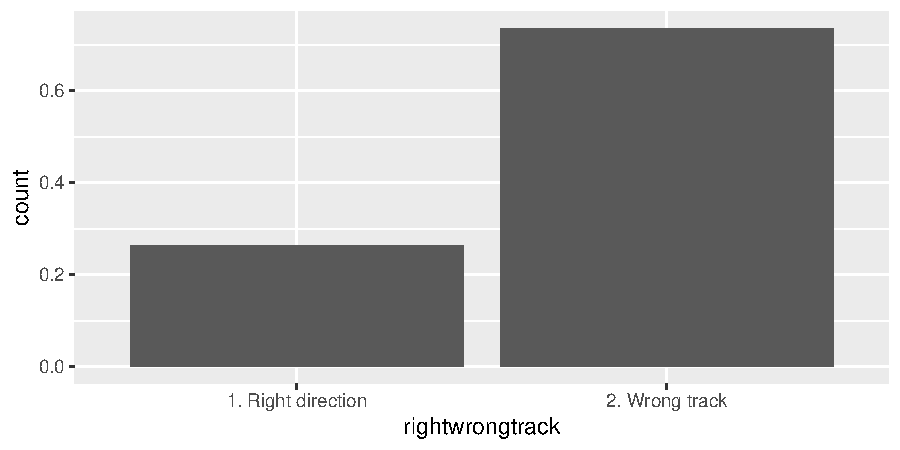
\includegraphics[width=0.95\linewidth]{figure/unnamed-chunk-44-1} 
\end{knitrout}

\end{frame}
\begin{frame}[fragile]{Example 8A: Adding titles to previous plot}
\begin{knitrout}
\definecolor{shadecolor}{rgb}{0.969, 0.969, 0.969}\color{fgcolor}\begin{kframe}
\begin{alltt}
\hlstd{plot8atitle} \hlkwb{=} \hlstd{plot8a} \hlopt{+} \hlkwd{ggtitle}\hlstd{(}\hlstr{"Right Direction / Wrong Track"}\hlstd{)} \hlopt{+}
    \hlkwd{ylab}\hlstd{(}\hlstr{"Proportion"}\hlstd{)}
\end{alltt}
\end{kframe}
\end{knitrout}
\end{frame}


\begin{frame}[fragile]{Example 8A: Adding titles to previous plot}
\begin{knitrout}
\definecolor{shadecolor}{rgb}{0.969, 0.969, 0.969}\color{fgcolor}\begin{kframe}
\begin{alltt}
\hlstd{plot8atitle}
\end{alltt}
\end{kframe}
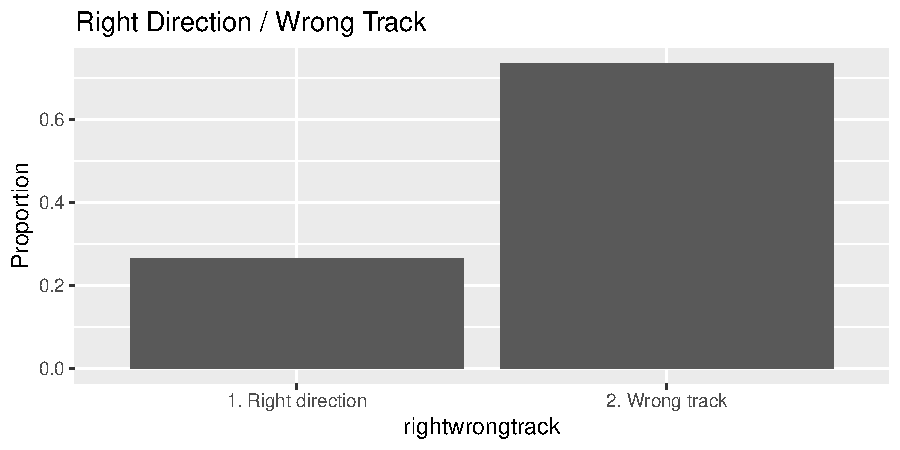
\includegraphics[width=0.95\linewidth]{figure/unnamed-chunk-46-1} 
\end{knitrout}
\end{frame}
\begin{frame}[fragile]{Example 8B: ggsurvey Bar Chart with Survey Object }
\begin{knitrout}
\definecolor{shadecolor}{rgb}{0.969, 0.969, 0.969}\color{fgcolor}\begin{kframe}
\begin{alltt}
\hlstd{plot8b} \hlkwb{=} \hlkwd{ggbarweight_svy}\hlstd{(anes_survey,}
    \hlstd{rightwrongtrack)}
\hlstd{plot8b}
\end{alltt}
\end{kframe}
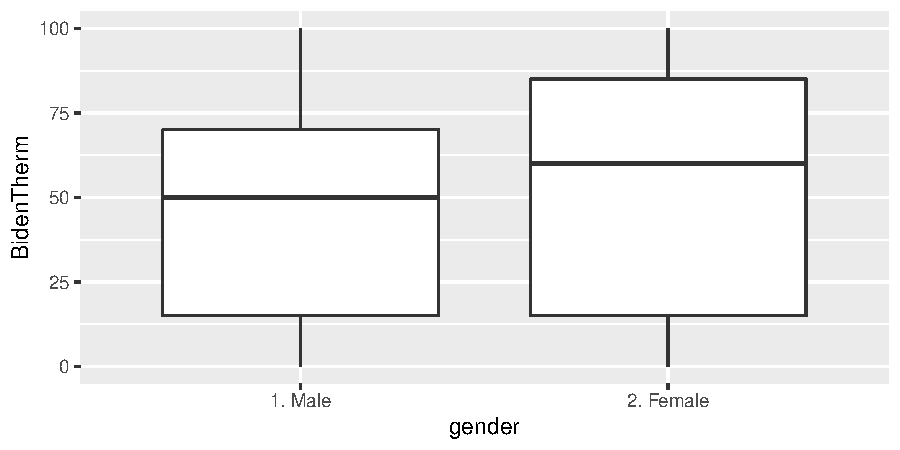
\includegraphics[width=0.95\linewidth]{figure/unnamed-chunk-47-1} 
\end{knitrout}
\end{frame}
\begin{frame}[fragile]{Example 8B: Adding titles to previous plot}

\begin{knitrout}
\definecolor{shadecolor}{rgb}{0.969, 0.969, 0.969}\color{fgcolor}\begin{kframe}
\begin{alltt}
\hlstd{plot8title} \hlkwb{=} \hlstd{plot8b} \hlopt{+} \hlkwd{ggtitle}\hlstd{(}\hlstr{"Right Direction / Wrong Track"}\hlstd{)} \hlopt{+}
    \hlkwd{xlab}\hlstd{(}\hlstr{"Proportion"}\hlstd{)}
\end{alltt}
\end{kframe}
\end{knitrout}

\end{frame}
\begin{frame}[fragile]{Example 8B: Adding titles to previous plot}

\begin{knitrout}
\definecolor{shadecolor}{rgb}{0.969, 0.969, 0.969}\color{fgcolor}\begin{kframe}
\begin{alltt}
\hlstd{plot8title}
\end{alltt}
\end{kframe}
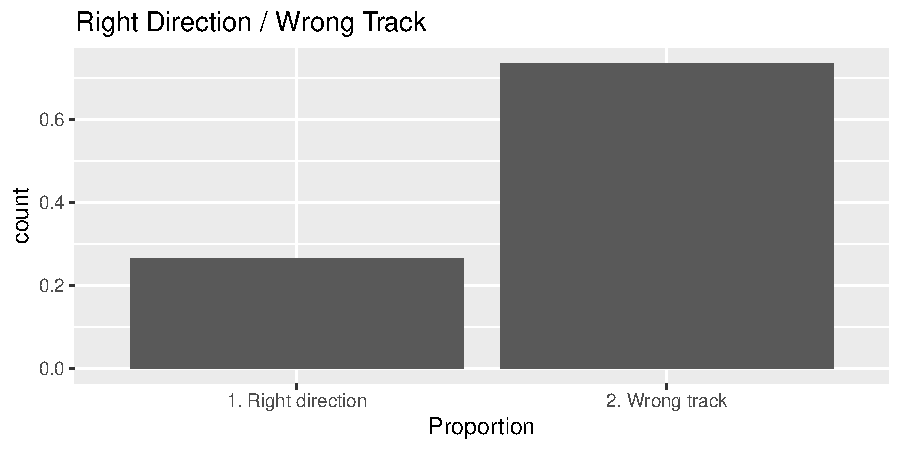
\includegraphics[width=0.95\linewidth]{figure/unnamed-chunk-49-1} 
\end{knitrout}

\end{frame}

\begin{frame}{Filtering: Advanced}
Sometimes we don't want to include a certain category in the plot.  For instance we may want to remove the refusals from the graph. We can use the filter  function from dplyr on a data frame to remove the refusals from the plot, and then pipe operator. The pipe operator passes the object on the left of the pipe into the function on the right as the first argument. At this time this only works with data frames with survey weights.
\end{frame}

\begin{frame}[fragile]{Removing Refusals and Don't Know}
\begin{knitrout}
\definecolor{shadecolor}{rgb}{0.969, 0.969, 0.969}\color{fgcolor}\begin{kframe}
\begin{alltt}
\hlstd{filterplot} \hlkwb{=} \hlstd{timeseries_2020} \hlopt
    \hlkwd{filter}\hlstd{(race} \hlopt{==} \hlstr{"1. White, non-Hispanic"}\hlstd{)} \hlopt
    \hlkwd{ggbarweight}\hlstd{(rightwrongtrack,}
        \hlstd{V200010a)}
\end{alltt}
\end{kframe}
\end{knitrout}

\end{frame}

\begin{frame}[fragile]{Removing Refusals and Don't Know}
\begin{knitrout}
\definecolor{shadecolor}{rgb}{0.969, 0.969, 0.969}\color{fgcolor}\begin{kframe}
\begin{alltt}
\hlstd{filterplot}
\end{alltt}
\end{kframe}
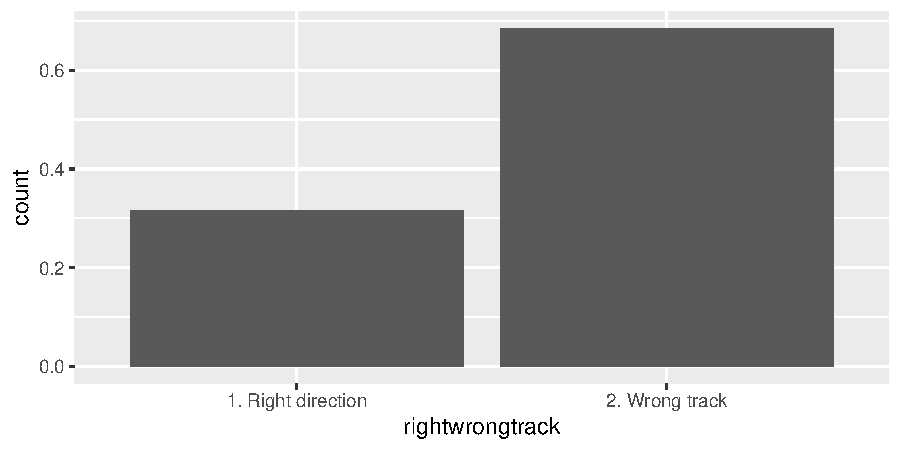
\includegraphics[width=0.95\linewidth]{figure/unnamed-chunk-51-1} 
\end{knitrout}

\end{frame}


\begin{frame}[fragile]{Example 9A: Bar Chart with One Crosstab For Dataframe}
Sometimes the text overlaps in ggplots.
\begin{knitrout}
\definecolor{shadecolor}{rgb}{0.969, 0.969, 0.969}\color{fgcolor}\begin{kframe}
\begin{alltt}
\hlkwd{ggbarcrosstabs}\hlstd{(timeseries_2020,}
    \hlstd{rightwrongtrack, gender, V200010a)}
\end{alltt}
\end{kframe}
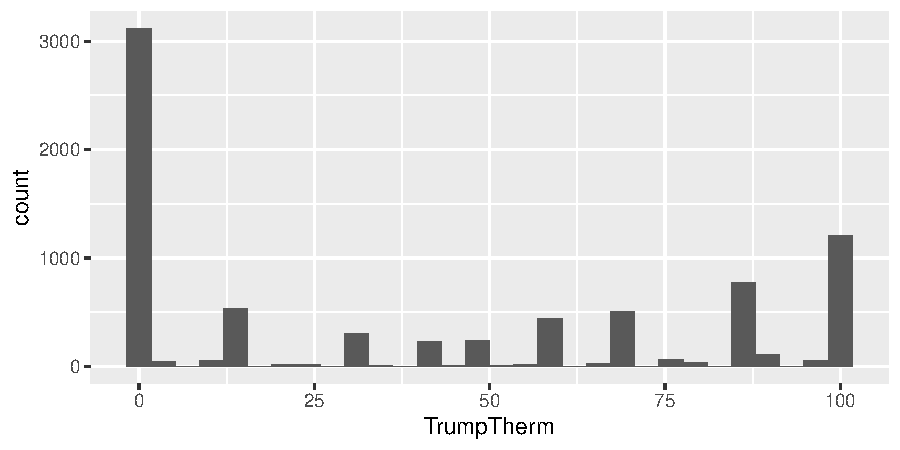
\includegraphics[width=0.95\linewidth]{figure/unnamed-chunk-52-1} 
\end{knitrout}
\end{frame}

\begin{frame}[fragile]{Example 9A: Text Wrap Labels}
We can use the stringr package to use text wrapping for the labels on the bars.
\begin{knitrout}
\definecolor{shadecolor}{rgb}{0.969, 0.969, 0.969}\color{fgcolor}\begin{kframe}
\begin{alltt}
\hlkwd{library}\hlstd{(stringr)}
\hlstd{plot9Atext} \hlkwb{=} \hlkwd{ggbarcrosstabs}\hlstd{(timeseries_2020,}
    \hlstd{rightwrongtrack, gender, V200010a)} \hlopt{+}
    \hlkwd{scale_x_discrete}\hlstd{(}\hlkwc{labels} \hlstd{=} \hlkwa{function}\hlstd{(}\hlkwc{x}\hlstd{)} \hlkwd{str_wrap}\hlstd{(x,}
        \hlkwc{width} \hlstd{=} \hlnum{10}\hlstd{))}
\end{alltt}
\end{kframe}
\end{knitrout}
\end{frame}

\begin{frame}[fragile]{Example 9A: Text Wrap Labels}
We can use the stringr package to use text wrapping for the labels on the bars.
\begin{knitrout}
\definecolor{shadecolor}{rgb}{0.969, 0.969, 0.969}\color{fgcolor}\begin{kframe}
\begin{alltt}
\hlkwd{library}\hlstd{(stringr)}
\hlstd{plot9Atext}
\end{alltt}
\end{kframe}
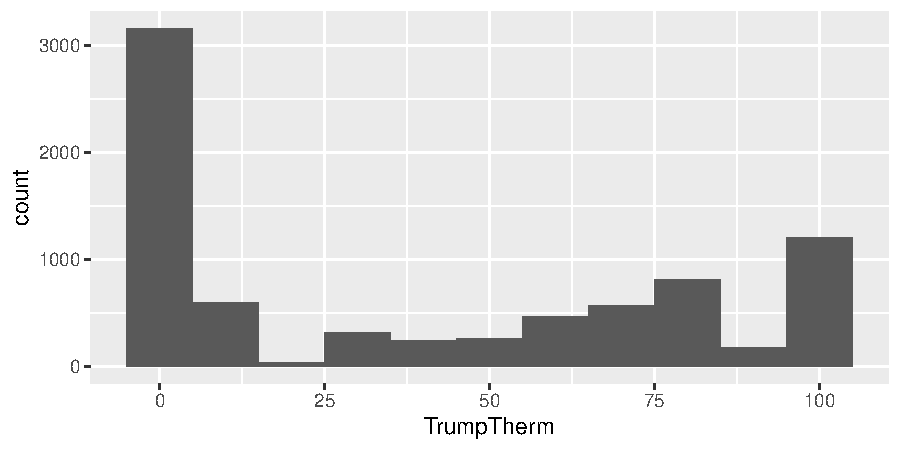
\includegraphics[width=0.95\linewidth]{figure/unnamed-chunk-54-1} 
\end{knitrout}
\end{frame}

\begin{frame}[fragile]{Example 9B: Bar Chart with One Crosstab For svydesign}

\begin{knitrout}
\definecolor{shadecolor}{rgb}{0.969, 0.969, 0.969}\color{fgcolor}\begin{kframe}
\begin{alltt}
\hlkwd{ggbarcrosstabs_svy}\hlstd{(anes_survey,}
    \hlstd{rightwrongtrack, gender)}
\end{alltt}
\end{kframe}
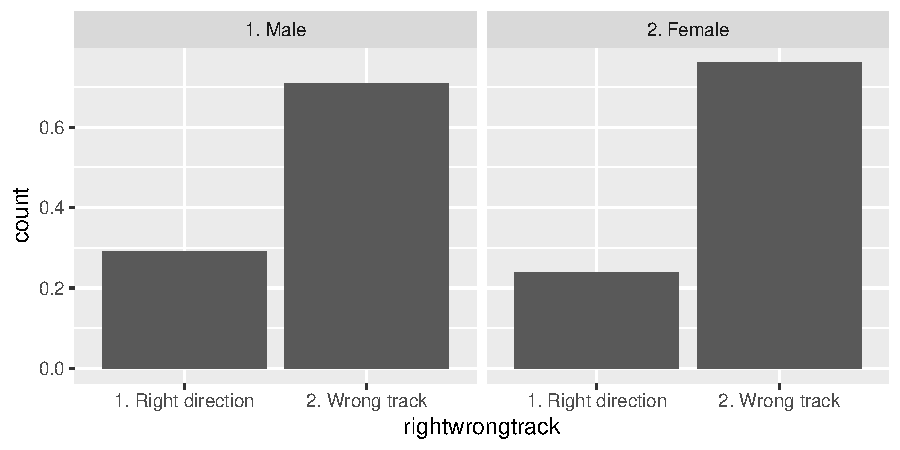
\includegraphics[width=0.95\linewidth]{figure/unnamed-chunk-55-1} 
\end{knitrout}
\end{frame}

\begin{frame}[fragile]{Example 9B: Text Wrap Labels}

\begin{knitrout}
\definecolor{shadecolor}{rgb}{0.969, 0.969, 0.969}\color{fgcolor}\begin{kframe}
\begin{alltt}
\hlkwd{ggbarcrosstabs_svy}\hlstd{(anes_survey,}
    \hlstd{rightwrongtrack, gender)} \hlopt{+}
    \hlkwd{scale_x_discrete}\hlstd{(}\hlkwc{labels} \hlstd{=} \hlkwa{function}\hlstd{(}\hlkwc{x}\hlstd{)} \hlkwd{str_wrap}\hlstd{(x,}
        \hlkwc{width} \hlstd{=} \hlnum{10}\hlstd{))}
\end{alltt}
\end{kframe}
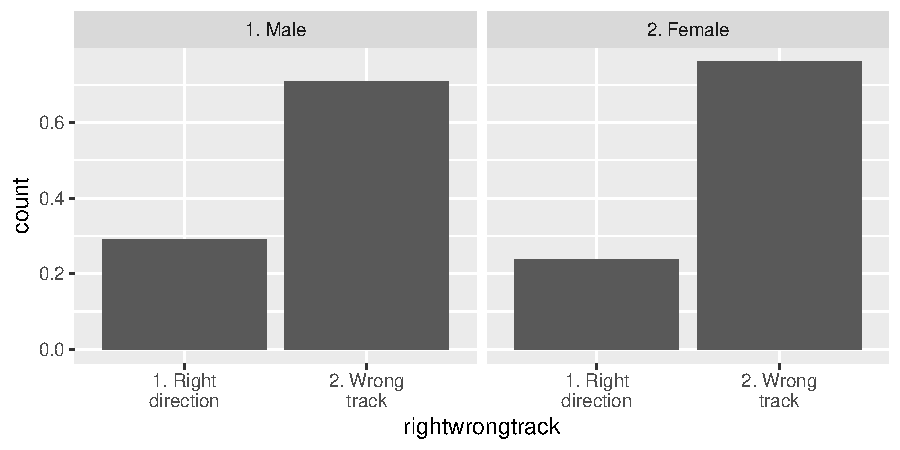
\includegraphics[width=0.95\linewidth]{figure/unnamed-chunk-56-1} 
\end{knitrout}
\end{frame}


\begin{frame}[fragile]{Example 10A: Bar Chart with Two Crosstab For Dataframe}

\begin{knitrout}
\definecolor{shadecolor}{rgb}{0.969, 0.969, 0.969}\color{fgcolor}\begin{kframe}
\begin{alltt}
\hlstd{plot10A} \hlkwb{=} \hlkwd{ggbarcrosstabs3d}\hlstd{(timeseries_2020,}
    \hlstd{rightwrongtrack, economy, gender,}
    \hlstd{V200010a)}
\end{alltt}
\end{kframe}
\end{knitrout}
\end{frame}

\begin{frame}[fragile]{Example 10A: Bar Chart with Two Crosstab For Dataframe}

\begin{knitrout}
\definecolor{shadecolor}{rgb}{0.969, 0.969, 0.969}\color{fgcolor}\begin{kframe}
\begin{alltt}
\hlstd{plot10A}
\end{alltt}
\end{kframe}
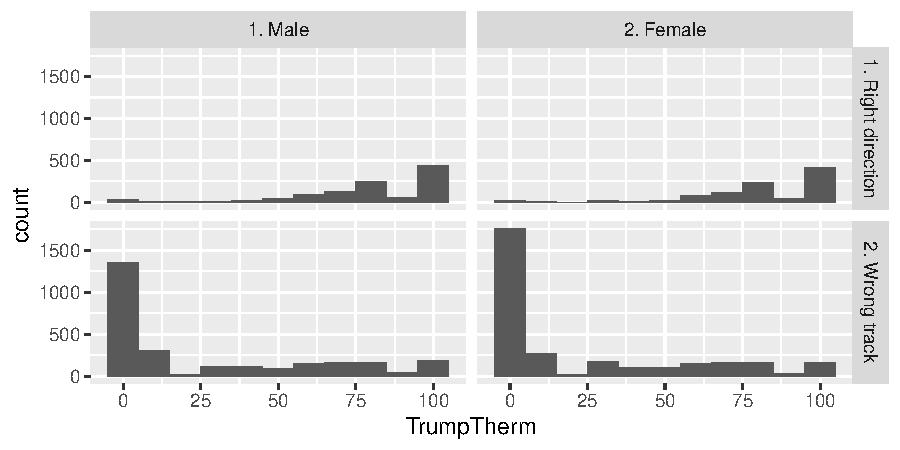
\includegraphics[width=0.95\linewidth]{figure/unnamed-chunk-58-1} 
\end{knitrout}
\end{frame}

\begin{frame}[fragile]{Example 10A: Add Text Wrap Labels}

\begin{knitrout}
\definecolor{shadecolor}{rgb}{0.969, 0.969, 0.969}\color{fgcolor}\begin{kframe}
\begin{alltt}
\hlstd{plot10Atext} \hlkwb{=} \hlkwd{ggbarcrosstabs3d}\hlstd{(timeseries_2020,}
    \hlstd{rightwrongtrack, economy, gender,}
    \hlstd{V200010a,} \hlkwc{labeller} \hlstd{=} \hlkwd{label_wrap_gen}\hlstd{(}\hlkwc{width} \hlstd{=} \hlnum{3}\hlstd{,}
        \hlkwc{multi_line} \hlstd{=} \hlnum{TRUE}\hlstd{))} \hlopt{+} \hlkwd{scale_x_discrete}\hlstd{(}\hlkwc{labels} \hlstd{=} \hlkwa{function}\hlstd{(}\hlkwc{x}\hlstd{)} \hlkwd{str_wrap}\hlstd{(x,}
    \hlkwc{width} \hlstd{=} \hlnum{10}\hlstd{))}
\end{alltt}
\end{kframe}
\end{knitrout}
\end{frame}

\begin{frame}[fragile]{Example 10A: Add Text Wrap Labels}

\begin{knitrout}
\definecolor{shadecolor}{rgb}{0.969, 0.969, 0.969}\color{fgcolor}\begin{kframe}
\begin{alltt}
\hlstd{plot10Atext}
\end{alltt}
\end{kframe}
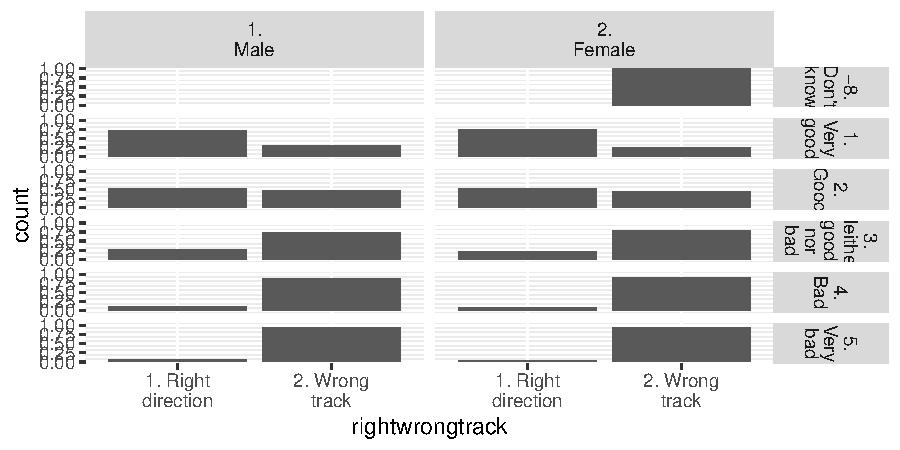
\includegraphics[width=0.95\linewidth]{figure/unnamed-chunk-60-1} 
\end{knitrout}
\end{frame}




\begin{frame}[fragile]{Example 10B: Bar chart with Two Crosstabs For svydesign}

\begin{knitrout}
\definecolor{shadecolor}{rgb}{0.969, 0.969, 0.969}\color{fgcolor}\begin{kframe}
\begin{alltt}
\hlkwd{ggbarcrosstabs3d_svy}\hlstd{(anes_survey,}
    \hlstd{rightwrongtrack, economy, gender)}
\end{alltt}
\end{kframe}
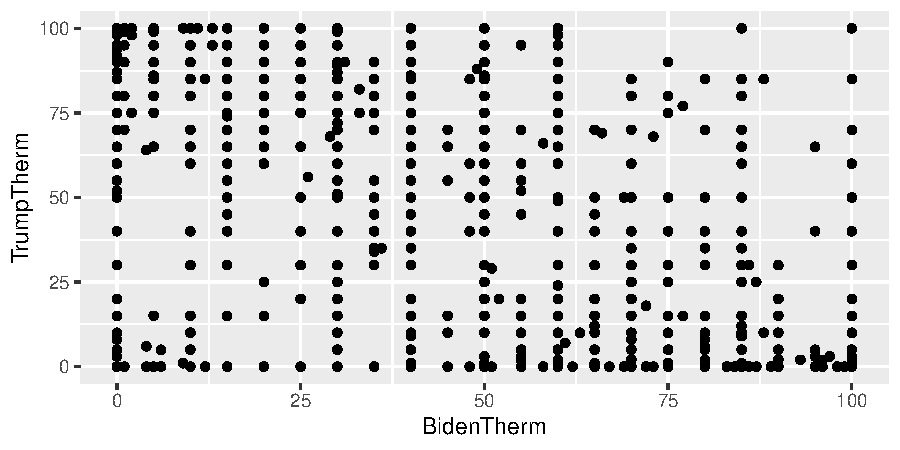
\includegraphics[width=0.95\linewidth]{figure/unnamed-chunk-61-1} 
\end{knitrout}
\end{frame}

\begin{frame}[fragile]{Example 10B: Text Wrap Labels}

\begin{knitrout}
\definecolor{shadecolor}{rgb}{0.969, 0.969, 0.969}\color{fgcolor}\begin{kframe}
\begin{alltt}
\hlkwd{ggbarcrosstabs3d_svy}\hlstd{(anes_survey,}
    \hlstd{rightwrongtrack, economy, gender,}
    \hlkwc{labeller} \hlstd{=} \hlkwd{label_wrap_gen}\hlstd{(}\hlkwc{width} \hlstd{=} \hlnum{3}\hlstd{,}
        \hlkwc{multi_line} \hlstd{=} \hlnum{TRUE}\hlstd{))} \hlopt{+} \hlkwd{scale_x_discrete}\hlstd{(}\hlkwc{labels} \hlstd{=} \hlkwa{function}\hlstd{(}\hlkwc{x}\hlstd{)} \hlkwd{str_wrap}\hlstd{(x,}
    \hlkwc{width} \hlstd{=} \hlnum{3}\hlstd{))}
\end{alltt}
\end{kframe}
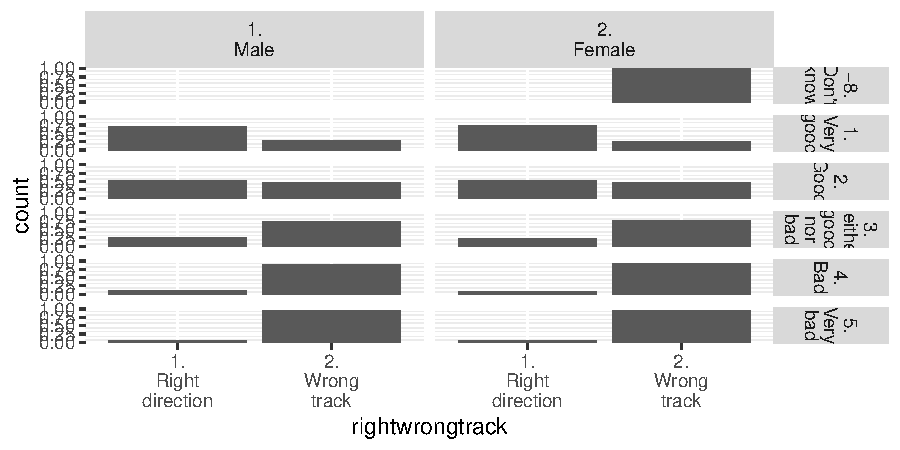
\includegraphics[width=0.95\linewidth]{figure/unnamed-chunk-62-1} 
\end{knitrout}
\end{frame}

\begin{frame}{Any Questions?}
\end{frame}

\section{Using ggsurvey for box plots}

\begin{frame}[fragile]{Box Plots}
A Boxplot is a way to visualize the distribution of a numeric variable such as a feeling thermometer. A boxplot highlights 5 key statistics: the minimum value, the 25th percentile, the median, the 75th percentile and the maximum value. In ggplot extreme values deemed to be outliers are marked with a dot. We will use the feeling thermometers for Joe Biden (V201151) and Donald Trump (V201152) in the 2020 ANES.


\end{frame}
\begin{frame}[fragile]{Process Data}
We need to first remove the refusals and convert the factor to a numeric in the data frame.
\begin{knitrout}
\definecolor{shadecolor}{rgb}{0.969, 0.969, 0.969}\color{fgcolor}\begin{kframe}
\begin{alltt}
\hlstd{timeseries_2020}\hlopt{$}\hlstd{BidenTherm} \hlkwb{=} \hlkwd{as.numeric}\hlstd{(}\hlkwd{as.character}\hlstd{(}
  \hlstd{timeseries_2020}\hlopt{$}\hlstd{V201151))}
\hlstd{timeseries_2020}\hlopt{$}\hlstd{TrumpTherm} \hlkwb{=} \hlkwd{as.numeric}\hlstd{(}\hlkwd{as.character}\hlstd{(}
  \hlstd{timeseries_2020}\hlopt{$}\hlstd{V201152))}
\hlstd{anes_svy}  \hlkwb{=} \hlstd{anes_svy} \hlopt \hlkwd{mutate}\hlstd{(}\hlkwc{BidenTherm} \hlstd{=}
\hlkwd{as.numeric}\hlstd{(}\hlkwd{as.character}\hlstd{(timeseries_2020}\hlopt{$}\hlstd{V201151)))}
\hlstd{anes_svy}  \hlkwb{=} \hlstd{anes_svy} \hlopt \hlkwd{mutate}\hlstd{(}\hlkwc{TrumpTherm} \hlstd{=}
\hlkwd{as.numeric}\hlstd{(}\hlkwd{as.character}\hlstd{(timeseries_2020}\hlopt{$}\hlstd{V201152)))}
\end{alltt}
\end{kframe}
\end{knitrout}
\end{frame}


\begin{frame}{ggsurvey boxplot Functions}
\begin{table}[]
\begin{tabular}{|l|l|l|}
\hline
Plot type                                                        & Data type  & ggsurvey function                    \\ \hline
Box Plot                                                         & data frame & ggboxweight(df, x, weights)          \\ \hline
Box Plot                                                         & svydesign  & ggboxweight\_svy(surveyobj, x)       \\ \hline
\begin{tabular}[c]{@{}l@{}}Box plot \\ with 1 Facet\end{tabular} & data frame & ggboxweight2d(df, x, y,weights)      \\ \hline
\begin{tabular}[c]{@{}l@{}}Box plot\\ with 1 Facet\end{tabular}  & svydesign  & ggboxweight2d\_svy(surveyobj, x, y)  \\ \hline
\begin{tabular}[c]{@{}l@{}}Box plot\\ with 2 Facets\end{tabular}  & data frame & ggboxweight3d(df, x, y,z weights)    \\ \hline
\begin{tabular}[c]{@{}l@{}}Box plot\\ with 2 Facets\end{tabular}  & svydesign  & ggboxweight3d\_svy(surveyobj, x,y,z) \\ \hline
\end{tabular}
\end{table}
\end{frame}

\begin{frame}[fragile]{Example 11A: Boxplot with data frame object}
\begin{knitrout}
\definecolor{shadecolor}{rgb}{0.969, 0.969, 0.969}\color{fgcolor}\begin{kframe}
\begin{alltt}
\hlkwd{ggboxweight}\hlstd{(timeseries_2020, BidenTherm,}
    \hlstd{V200010a)}
\end{alltt}
\end{kframe}
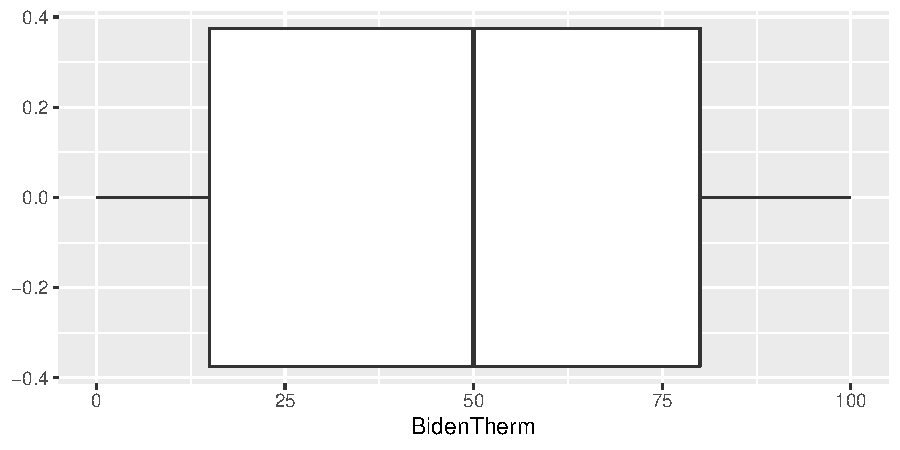
\includegraphics[width=0.95\linewidth]{figure/unnamed-chunk-64-1} 
\end{knitrout}

\end{frame}

\begin{frame}[fragile]{Example 11B: Boxplot with survey design object}
Recall that we stored the survey design object for th ANES in anes\_svy.
\begin{knitrout}
\definecolor{shadecolor}{rgb}{0.969, 0.969, 0.969}\color{fgcolor}\begin{kframe}
\begin{alltt}
\hlkwd{ggboxweight_svy}\hlstd{(anes_svy, BidenTherm)}
\end{alltt}
\end{kframe}
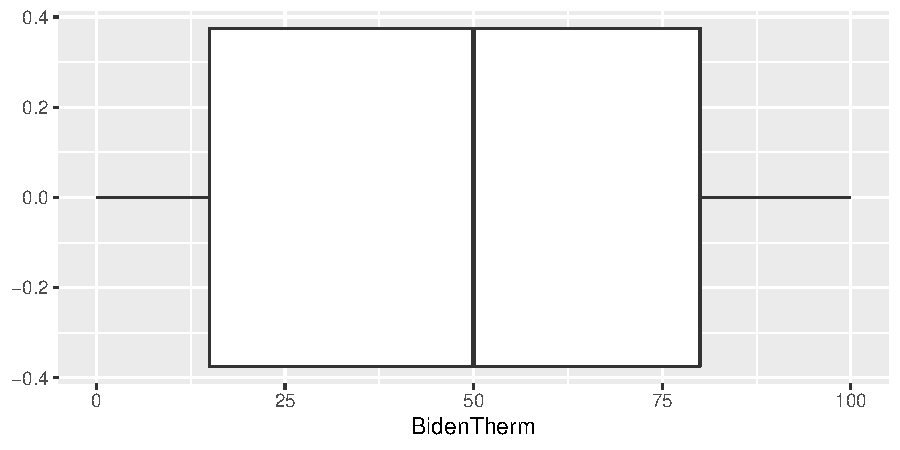
\includegraphics[width=0.95\linewidth]{figure/unnamed-chunk-65-1} 
\end{knitrout}

\end{frame}


\begin{frame}[fragile]{Example 12A: Boxplot with one facet with data frame object}
\begin{knitrout}
\definecolor{shadecolor}{rgb}{0.969, 0.969, 0.969}\color{fgcolor}\begin{kframe}
\begin{alltt}
\hlkwd{ggboxweight2d}\hlstd{(timeseries_2020,}
    \hlstd{BidenTherm, gender, V200010a)}
\end{alltt}
\end{kframe}
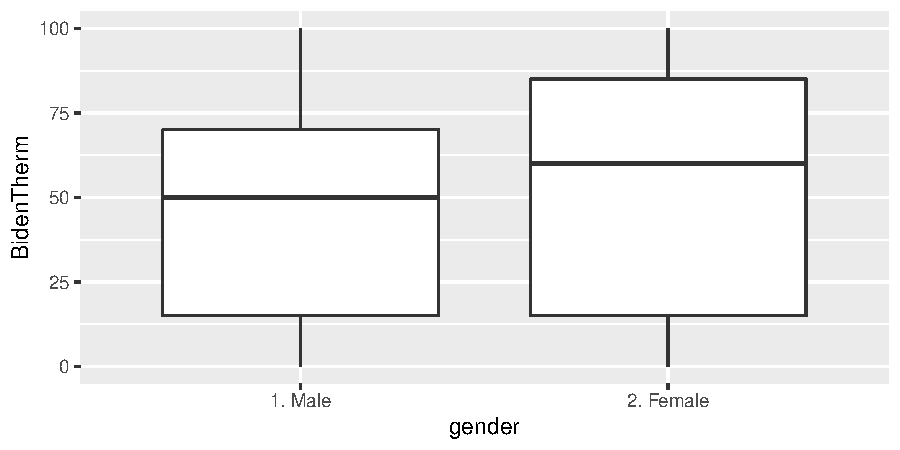
\includegraphics[width=0.95\linewidth]{figure/unnamed-chunk-66-1} 
\end{knitrout}
\end{frame}

\begin{frame}[fragile]{Example 12B: Boxplot with one facet with survey design object}
\begin{knitrout}
\definecolor{shadecolor}{rgb}{0.969, 0.969, 0.969}\color{fgcolor}\begin{kframe}
\begin{alltt}
\hlkwd{ggboxweight2d_svy}\hlstd{(anes_svy, BidenTherm,}
    \hlstd{gender)} \hlopt{+} \hlkwd{ggtitle}\hlstd{(}\hlstr{"Biden Feeling Thermometer by Gender"}\hlstd{)}
\end{alltt}
\end{kframe}
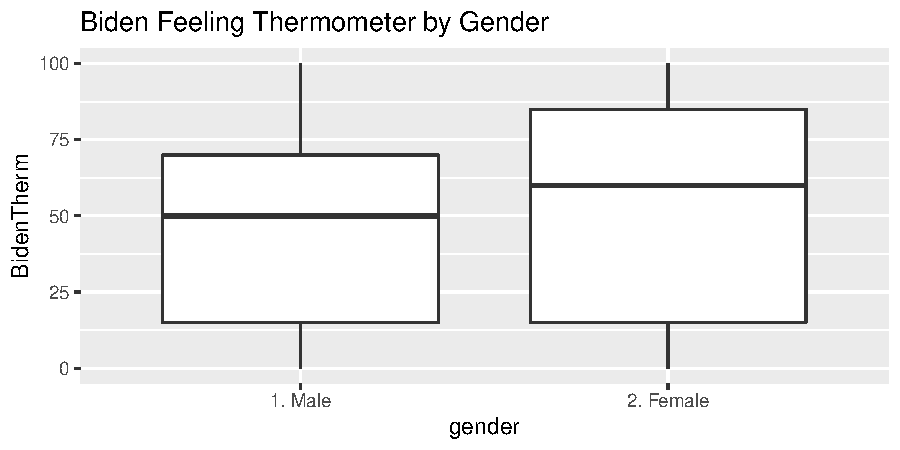
\includegraphics[width=0.95\linewidth]{figure/unnamed-chunk-67-1} 
\end{knitrout}

\end{frame}

\begin{frame}[fragile]{Example 12A: Boxplot with two facets with data frame object}
\begin{knitrout}
\definecolor{shadecolor}{rgb}{0.969, 0.969, 0.969}\color{fgcolor}\begin{kframe}
\begin{alltt}
\hlkwd{ggboxweight3d}\hlstd{(timeseries_2020,}
    \hlstd{BidenTherm, rightwrongtrack,}
    \hlstd{gender, V200010a)}
\end{alltt}
\end{kframe}
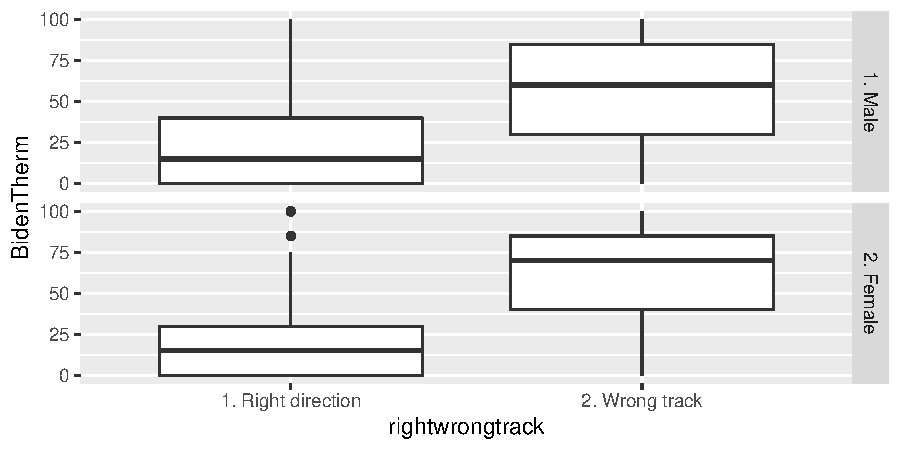
\includegraphics[width=0.95\linewidth]{figure/unnamed-chunk-68-1} 
\end{knitrout}

\end{frame}

\begin{frame}[fragile]{Example 12B: Boxplot with two facets with survey design object}
\begin{knitrout}
\definecolor{shadecolor}{rgb}{0.969, 0.969, 0.969}\color{fgcolor}\begin{kframe}
\begin{alltt}
\hlkwd{ggboxweight3d_svy}\hlstd{(anes_svy, BidenTherm,}
    \hlstd{rightwrongtrack, gender)} \hlopt{+}
    \hlkwd{ggtitle}\hlstd{(}\hlstr{"Biden Feeling Thermometer by Gender"}\hlstd{)}
\end{alltt}
\end{kframe}
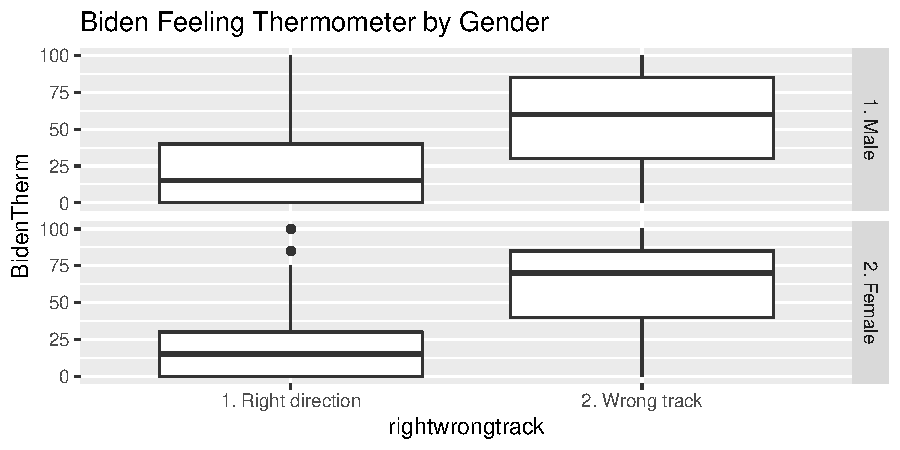
\includegraphics[width=0.95\linewidth]{figure/unnamed-chunk-69-1} 
\end{knitrout}

\end{frame}

\begin{frame}[fragile]{Base ggplot solution for 12A}
\begin{knitrout}
\definecolor{shadecolor}{rgb}{0.969, 0.969, 0.969}\color{fgcolor}\begin{kframe}
\begin{alltt}
\hlkwd{ggplot}\hlstd{(timeseries_2020,} \hlkwd{aes}\hlstd{(}\hlkwc{x} \hlstd{= rightwrongtrack,}
    \hlkwc{y} \hlstd{= BidenTherm))} \hlopt{+} \hlkwd{geom_boxplot}\hlstd{(}\hlkwd{aes}\hlstd{(}\hlkwc{weight} \hlstd{= V200010a))} \hlopt{+}
    \hlkwd{facet_grid}\hlstd{(}\hlkwc{rows} \hlstd{=} \hlkwd{vars}\hlstd{(gender))}
\end{alltt}
\end{kframe}
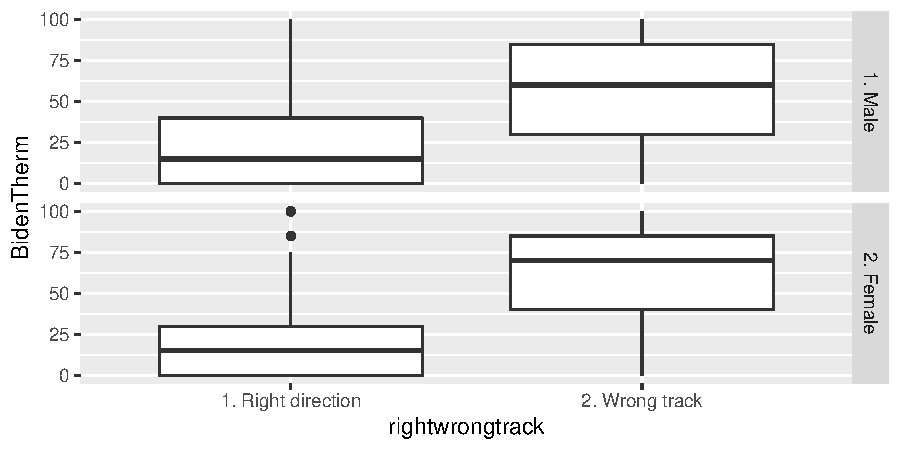
\includegraphics[width=0.95\linewidth]{figure/unnamed-chunk-70-1} 
\end{knitrout}

\end{frame}
\begin{frame}{Any Questions?}
\end{frame}
\section{Using ggsurvey for histograms}
\begin{frame}{Histograms in ggsurvey}
We will work with Trump'a feeling thermometer question to make histograms.
\begin{table}[]
\begin{tabular}{|l|l|l|}
\hline
Plot type                                                        & Data type  & ggsurvey function                     \\ \hline
Histogram                                                        & data frame & gghistweight(df,x,weights,binwidth)          \\ \hline
Histogram                                                        & svydesign  & gghistweight\_svy(surveyobj,x,binwidth)       \\ \hline
\begin{tabular}[c]{@{}l@{}}Histogram\\ with 1 Facet\end{tabular} & data frame & gghistweight2d(df,x,y,weights,binwidth)      \\ \hline
\begin{tabular}[c]{@{}l@{}}Histogram\\ with 1 Facet\end{tabular} & svydesign  & gghistweight2d\_svy(surveyobj,x,y,binwidth)  \\ \hline
\begin{tabular}[c]{@{}l@{}}Histogram\\ with 2 Facets\end{tabular} & data frame & gghistweight3d(df,x, y,z,weights,binwidth)    \\ \hline
\begin{tabular}[c]{@{}l@{}}Histogram\\ with 2 Facets\end{tabular} & svydesign  & gghistweight3d\_svy(surveyobj,x,y,z,binwidth) \\ \hline
\end{tabular}
\end{table}
\end{frame}

\begin{frame}[fragile]{Example 13A: Histogram with data frame object}
\begin{knitrout}
\definecolor{shadecolor}{rgb}{0.969, 0.969, 0.969}\color{fgcolor}\begin{kframe}
\begin{alltt}
\hlkwd{gghistweight}\hlstd{(timeseries_2020, TrumpTherm,}
    \hlstd{V200010a)}
\end{alltt}
\end{kframe}
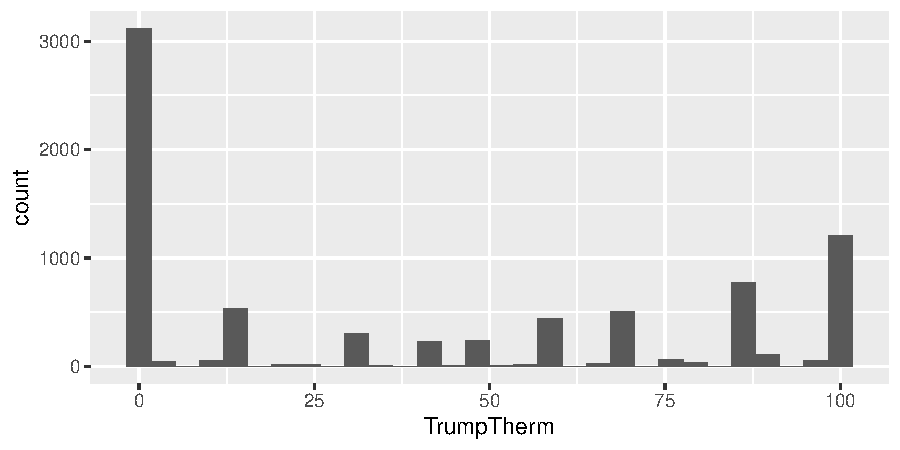
\includegraphics[width=0.95\linewidth]{figure/unnamed-chunk-71-1} 
\end{knitrout}

\end{frame}

\begin{frame}[fragile]{Example 13A: Histogram with data frame object}
Try a binwidth of 5.
\begin{knitrout}
\definecolor{shadecolor}{rgb}{0.969, 0.969, 0.969}\color{fgcolor}\begin{kframe}
\begin{alltt}
\hlkwd{gghistweight}\hlstd{(timeseries_2020, TrumpTherm,}
    \hlstd{V200010a,} \hlkwc{binwidth} \hlstd{=} \hlnum{5}\hlstd{)}
\end{alltt}
\end{kframe}
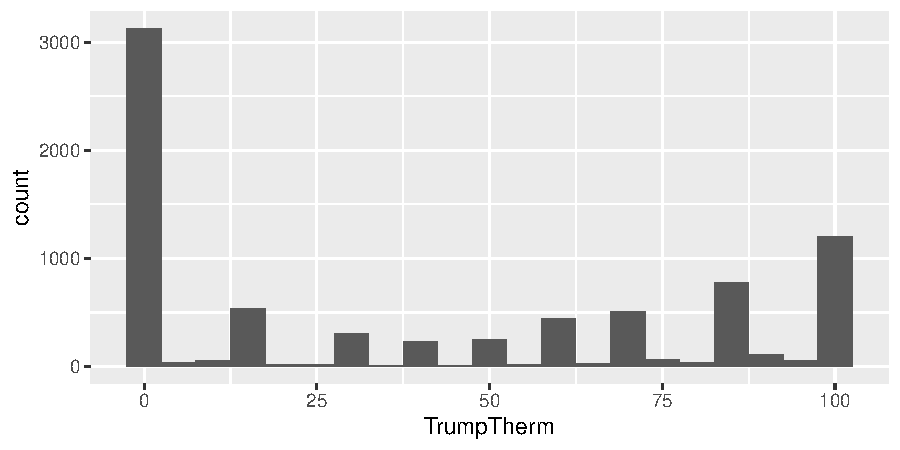
\includegraphics[width=0.95\linewidth]{figure/unnamed-chunk-72-1} 
\end{knitrout}

\end{frame}

\begin{frame}[fragile]{Example 13A: Histogram with data frame object}
Try a binwidth of 10. This is what I prefer, and will use in the next plots.
\begin{knitrout}
\definecolor{shadecolor}{rgb}{0.969, 0.969, 0.969}\color{fgcolor}\begin{kframe}
\begin{alltt}
\hlkwd{gghistweight}\hlstd{(timeseries_2020, TrumpTherm,}
    \hlstd{V200010a,} \hlkwc{binwidth} \hlstd{=} \hlnum{10}\hlstd{)}
\end{alltt}
\end{kframe}
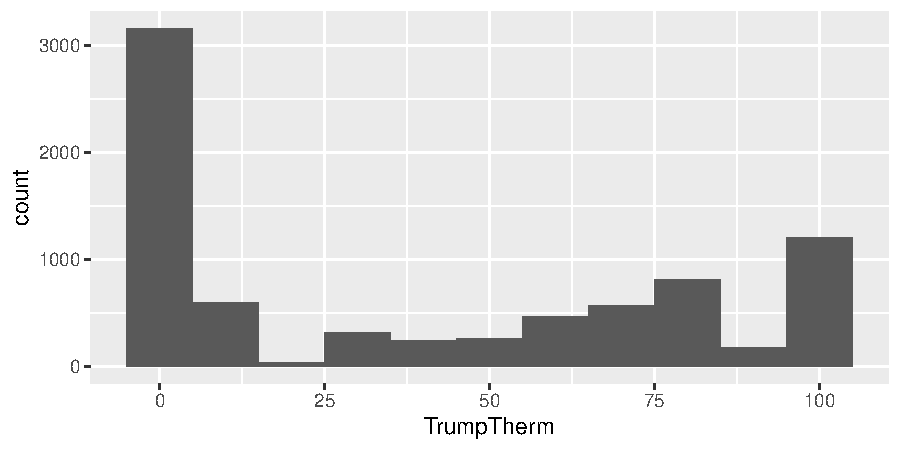
\includegraphics[width=0.95\linewidth]{figure/unnamed-chunk-73-1} 
\end{knitrout}

\end{frame}

\begin{frame}[fragile]{Example 13B: Histogram with survey design object}
Recall that we stored the survey design object for th ANES in anes\_svy.
\begin{knitrout}
\definecolor{shadecolor}{rgb}{0.969, 0.969, 0.969}\color{fgcolor}\begin{kframe}
\begin{alltt}
\hlkwd{gghistweight_svy}\hlstd{(anes_svy, TrumpTherm,}
    \hlkwc{binwidth} \hlstd{=} \hlnum{10}\hlstd{)}
\end{alltt}
\end{kframe}
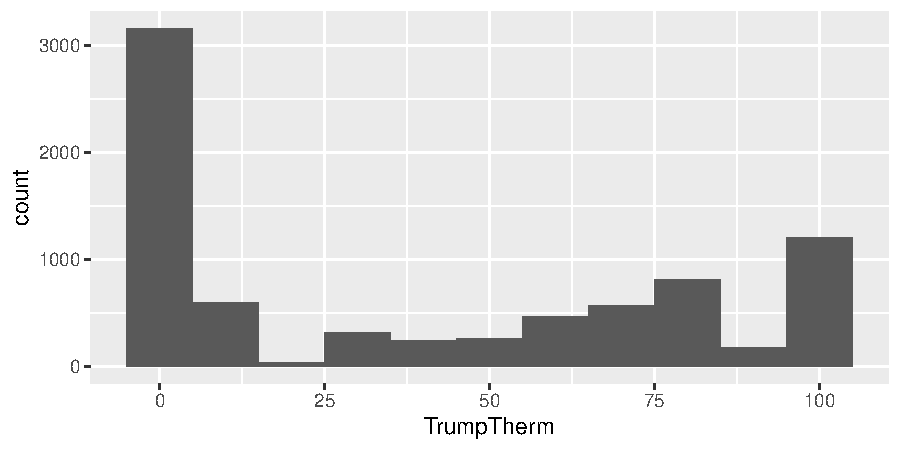
\includegraphics[width=0.95\linewidth]{figure/unnamed-chunk-74-1} 
\end{knitrout}

\end{frame}


\begin{frame}[fragile]{Example 14A: Histogram with one facet with data frame object}
\begin{knitrout}
\definecolor{shadecolor}{rgb}{0.969, 0.969, 0.969}\color{fgcolor}\begin{kframe}
\begin{alltt}
\hlkwd{gghistweight2d}\hlstd{(timeseries_2020,}
    \hlstd{TrumpTherm, gender, V200010a,}
    \hlkwc{binwidth} \hlstd{=} \hlnum{10}\hlstd{)}
\end{alltt}
\end{kframe}
\includegraphics[width=0.95\linewidth]{figure/unnamed-chunk-75-1} 
\end{knitrout}
\end{frame}

\begin{frame}[fragile]{Example 14B: Histogram with one facet with survey design object}
\begin{knitrout}
\definecolor{shadecolor}{rgb}{0.969, 0.969, 0.969}\color{fgcolor}\begin{kframe}
\begin{alltt}
\hlkwd{gghistweight2d_svy}\hlstd{(anes_svy, TrumpTherm,}
    \hlstd{gender,} \hlkwc{binwidth} \hlstd{=} \hlnum{10}\hlstd{)} \hlopt{+} \hlkwd{ggtitle}\hlstd{(}\hlstr{"Biden Feeling Thermometer by Gender"}\hlstd{)}
\end{alltt}
\end{kframe}
\includegraphics[width=0.95\linewidth]{figure/unnamed-chunk-76-1} 
\end{knitrout}

\end{frame}

\begin{frame}[fragile]{Example 15A: Histogram with two facets with data frame object}
\begin{knitrout}
\definecolor{shadecolor}{rgb}{0.969, 0.969, 0.969}\color{fgcolor}\begin{kframe}
\begin{alltt}
\hlkwd{gghistweight3d}\hlstd{(timeseries_2020,}
    \hlstd{TrumpTherm, rightwrongtrack,}
    \hlstd{gender, V200010a,} \hlkwc{binwidth} \hlstd{=} \hlnum{10}\hlstd{)}
\end{alltt}
\end{kframe}
\includegraphics[width=0.95\linewidth]{figure/unnamed-chunk-77-1} 
\end{knitrout}

\end{frame}

\begin{frame}[fragile]{Example 15B: Histogram with two facets with survey design object}
\begin{knitrout}
\definecolor{shadecolor}{rgb}{0.969, 0.969, 0.969}\color{fgcolor}\begin{kframe}
\begin{alltt}
\hlkwd{gghistweight3d_svy}\hlstd{(anes_svy, TrumpTherm,}
    \hlstd{rightwrongtrack, gender,} \hlkwc{binwidth} \hlstd{=} \hlnum{10}\hlstd{)}
\end{alltt}
\end{kframe}
\includegraphics[width=0.95\linewidth]{figure/unnamed-chunk-78-1} 
\end{knitrout}

\end{frame}

\begin{frame}[fragile]{Base ggplot solution for 15A}
\begin{knitrout}
\definecolor{shadecolor}{rgb}{0.969, 0.969, 0.969}\color{fgcolor}\begin{kframe}
\begin{alltt}
\hlkwd{ggplot}\hlstd{(timeseries_2020,} \hlkwd{aes}\hlstd{(TrumpTherm))} \hlopt{+}
    \hlkwd{geom_histogram}\hlstd{(}\hlkwd{aes}\hlstd{(}\hlkwc{weight} \hlstd{= V200010a),}
        \hlkwc{binwidth} \hlstd{=} \hlnum{10}\hlstd{)} \hlopt{+} \hlkwd{facet_grid}\hlstd{(}\hlkwc{rows} \hlstd{=} \hlkwd{vars}\hlstd{(gender))}
\end{alltt}
\end{kframe}
\includegraphics[width=0.95\linewidth]{figure/unnamed-chunk-79-1} 
\end{knitrout}

\end{frame}

\begin{frame}{Any Questions?}
\end{frame}
\section{Using ggsurvey for Hexplots}

\begin{frame}[fragile]{Motivation for Hexplot}
Sometimes you have multiple data points that overlap.  When we plot the Trump Feeling Thermometer by the Biden Feeling Thermometer we see less points than number of observations.
\begin{knitrout}
\definecolor{shadecolor}{rgb}{0.969, 0.969, 0.969}\color{fgcolor}\begin{kframe}
\begin{alltt}
\hlkwd{ggplot}\hlstd{(timeseries_2020,} \hlkwd{aes}\hlstd{(}\hlkwc{x} \hlstd{= BidenTherm,}
    \hlkwc{y} \hlstd{= TrumpTherm))} \hlopt{+} \hlkwd{geom_point}\hlstd{()}
\end{alltt}
\end{kframe}
\includegraphics[width=0.95\linewidth]{figure/unnamed-chunk-80-1} 
\begin{kframe}\begin{alltt}
\hlkwd{nrow}\hlstd{(timeseries_2020)}
\end{alltt}
\begin{verbatim}
## [1] 8066
\end{verbatim}
\end{kframe}
\end{knitrout}
\end{frame}

\begin{frame}[fragile]{Example 16A: Hexplot}
A hexplot creates bins of data that is close to overlapping and the intensity of shade in the bin denotes how many data points are in each bin. Ignoring survey weights this is done using the hexbin package.
\begin{knitrout}
\definecolor{shadecolor}{rgb}{0.969, 0.969, 0.969}\color{fgcolor}\begin{kframe}
\begin{alltt}
\hlkwd{library}\hlstd{(hexbin)}
\hlkwd{ggplot}\hlstd{(timeseries_2020,} \hlkwd{aes}\hlstd{(}\hlkwc{x} \hlstd{= BidenTherm,}
    \hlkwc{y} \hlstd{= TrumpTherm))} \hlopt{+} \hlkwd{geom_hex}\hlstd{()}
\end{alltt}
\end{kframe}
\includegraphics[width=0.95\linewidth]{figure/unnamed-chunk-81-1} 
\end{knitrout}


\end{frame}


\begin{frame}{Hexplot ggsurvey functions}
\begin{table}[]
\begin{tabular}{|l|l|l|}
\hline
Plot type                                                      & Data type  & ggsurvey function                    \\ \hline
Hexplot                                                        & data frame & gghexweight(df, x, y, weights)          \\ \hline
Hexplot                                                        & svydesign  & gghexweight\_svy(surveyobj, x, y)       \\ \hline
\begin{tabular}[c]{@{}l@{}}Hexplot\\ with 1 Facet\end{tabular} & data frame & gghexweight2d(df, x, y, z, weights)      \\ \hline
\begin{tabular}[c]{@{}l@{}}Hexplot\\ with 1 Facet\end{tabular} & svydesign  & gghexweight2d\_svy(surveyobj, x, y, z)  \\ \hline
\begin{tabular}[c]{@{}l@{}}Hexplot\\ with 2 Facet\end{tabular} & data frame & gghexweight3d(df, x, y, a, b weights)    \\ \hline
\begin{tabular}[c]{@{}l@{}}Hexplot\\ with 2 Facet\end{tabular} & svydesign  & gghexweight3d\_svy(surveyobj, x,y, a, b) \\ \hline
\end{tabular}
\end{table}
\end{frame}

\begin{frame}[fragile]{Example 16B: Weighted Hexplot With Dataframe}
In example 16 we did not account for the survey weights, but gghexweight does.
\begin{knitrout}
\definecolor{shadecolor}{rgb}{0.969, 0.969, 0.969}\color{fgcolor}\begin{kframe}
\begin{alltt}
\hlkwd{gghexweight}\hlstd{(timeseries_2020, BidenTherm,}
    \hlstd{TrumpTherm,} \hlkwc{weight} \hlstd{= V200010a)}
\end{alltt}
\end{kframe}
\includegraphics[width=0.95\linewidth]{figure/unnamed-chunk-82-1} 
\end{knitrout}

\end{frame}



\begin{frame}[fragile]{Example 16C: Using a Survey object}
In example 16 we did not account for the survey weights, but gghexweight does.
\begin{knitrout}
\definecolor{shadecolor}{rgb}{0.969, 0.969, 0.969}\color{fgcolor}\begin{kframe}
\begin{alltt}
\hlkwd{gghexweight_svy}\hlstd{(anes_svy, BidenTherm,}
    \hlstd{TrumpTherm)}
\end{alltt}
\end{kframe}
\includegraphics[width=0.95\linewidth]{figure/unnamed-chunk-83-1} 
\end{knitrout}

\end{frame}


\begin{frame}[fragile]{Example 17A: Weighted Hexplot with Facet For Data Frame}
\begin{knitrout}
\definecolor{shadecolor}{rgb}{0.969, 0.969, 0.969}\color{fgcolor}\begin{kframe}
\begin{alltt}
\hlkwd{gghexweight2d}\hlstd{(timeseries_2020,}
    \hlstd{BidenTherm, TrumpTherm, gender,}
    \hlkwc{weight} \hlstd{= V200010a)}
\end{alltt}
\end{kframe}
\includegraphics[width=0.95\linewidth]{figure/unnamed-chunk-84-1} 
\end{knitrout}

\end{frame}


\begin{frame}[fragile]{Example 17B: Weighted Hexplot with Facet For svydesign}

\begin{knitrout}
\definecolor{shadecolor}{rgb}{0.969, 0.969, 0.969}\color{fgcolor}\begin{kframe}
\begin{alltt}
\hlkwd{gghexweight2d_svy}\hlstd{(anes_svy, BidenTherm,}
    \hlstd{TrumpTherm, gender)}
\end{alltt}
\end{kframe}
\includegraphics[width=0.95\linewidth]{figure/unnamed-chunk-85-1} 
\end{knitrout}

\end{frame}


\begin{frame}[fragile]{Example 18A: Weighted Hexplot with facet}
\begin{knitrout}
\definecolor{shadecolor}{rgb}{0.969, 0.969, 0.969}\color{fgcolor}\begin{kframe}
\begin{alltt}
\hlkwd{gghexweight3d}\hlstd{(timeseries_2020,}
    \hlstd{BidenTherm, TrumpTherm, gender,}
    \hlstd{rightwrongtrack,} \hlkwc{weight} \hlstd{= V200010a)}
\end{alltt}
\end{kframe}
\includegraphics[width=0.95\linewidth]{figure/unnamed-chunk-86-1} 
\end{knitrout}

\end{frame}


\begin{frame}[fragile]{Example 18B: Weighted Hexplot with facet}

\begin{knitrout}
\definecolor{shadecolor}{rgb}{0.969, 0.969, 0.969}\color{fgcolor}\begin{kframe}
\begin{alltt}
\hlkwd{gghexweight3d_svy}\hlstd{(anes_svy, BidenTherm,}
    \hlstd{TrumpTherm, gender, rightwrongtrack)}
\end{alltt}
\end{kframe}
\includegraphics[width=0.95\linewidth]{figure/unnamed-chunk-87-1} 
\end{knitrout}

\end{frame}


\begin{frame}{Conclusion}
\begin{itemize}
\item ggsurvey is still in early development, and new features should be coming, including more customization for histograms
\item Full compatibility with srvyr is in progress.
\item In general ggsurvey is compatiable with most "add-on" functions from ggplot2 and related packages  (change color scheme, scales, titles), except geoms and facet\_grid.
\item ggplot2 and ggsurvey provide an open source way to create high quality visualizations of complex survey data
\item \href{https://github.com/balexanderstats/ggsurvey}{package website to download on your machine and follow updates}
\end{itemize}
\end{frame}

\begin{frame}{References}
\begin{itemize}
\item The \href{https://electionstudies.org/}{American National Election Studies} . These materials are based on work supported by the National Science Foundation under grant numbers SES 1444721, 2014-2017, the University of Michigan, and Stanford University.
\item Horst AM, Hill AP, Gorman KB (2020). \href{https://allisonhorst.github.io/palmerpenguins/}{palmerpenguins}: Palmer Archipelago (Antarctica) penguin data. R package version 0.1.0.
 doi:   10.5281/zenodo.3960218.
\item Hadley Wickham (2010) A Layered Grammar of Graphics, Journal of Computational and Graphical Statistics, 19:1, 3-28, DOI: 10.1198/jcgs.2009.07098

\end{itemize}
\end{frame}
\end{document}
